\documentclass{emulateapj}
%\documentclass[12pt,preprint]{aastex}

\usepackage{hyperref}

\usepackage{graphicx}
\usepackage{float}
\usepackage{amsmath}
\usepackage{epsfig,floatflt}
\usepackage{listings}
\usepackage{gensymb}
\usepackage{upgreek}
\usepackage{csquotes}
\usepackage{color}

\usepackage{bm}
\usepackage{blkarray}
% \usepackage{natbib}
% \setboolean{displaywatermark}{false}

\lstset{frame=tb,
  language=C++,
  aboveskip=3mm,
  belowskip=3mm,
  showstringspaces=false,
  columns=flexible,
  basicstyle={\small\ttfamily},
  numbers=none,
  numberstyle=\tiny\color{gray},
  keywordstyle=\color{blue},
  commentstyle=\color{dkgreen},
  stringstyle=\color{mauve},
  breaklines=true,
  breakatwhitespace=true,
  tabsize=3
}

\usepackage{hyperref}
\hypersetup{
    colorlinks=true,
    linkcolor=blue,
    filecolor=magenta,      
    urlcolor=blue,
    citecolor=blue,
}    

\newcommand\sini[0]{\sin{\theta}}
\newcommand\cosi[0]{\cos{\theta}}

\begin{document}

\title{Computational Physics - Project 2}

\author{
  Dahl, Jon Kristian \\
  \and
  Fløisand, Johan Andreas \\
  \and
  Sand, Mats Ola \\
}

% \maketitle
\begin{abstract}
With discretization and matrix representation we are able to utilize the potential of linear algebra to study one of the least intuitive branches of physics, namely quantum mechanics. We look at the fundemental example of an electron in a harmonic oscillator potential, as well as its neighbour; two electrons interacting in a potential (Coulomb and harmonic oscillator). We use the system's analytical solutions to give error estimations of the numerical methods used in this study. By matrix representing the double derivative and applying the harmonic oscillator potential, we identify the states of the electron as the eigenvectors of the matrix, and the electron energy levels as the corresponding eigenvalues. To get the eigendata, we use Jacobis eigenvalue algorithm. By replacing the distance parameter $r$ with a scaled dimensionless variable $\rho = r/\alpha$ and setting the matrix to be an $n \times n$ matrix, we find that the most precise numerical eigenvalues are found at $\rho \approx 6$ and $n = 400$, with the lowest minimum eigenvalue error value at $\approx 10^{-4}$ and the lowest maximum eigenvalue error value at $\approx 10^{-2}$, for a single electron system. For the two electron system we find that Jacobis method produce eigenvalues for the harmonic oscillator potential frequencies $\omega_r = 0.05$, $\omega_r = 0.25$ at $\lambda_1 = 0.3499996012$, $\lambda_2 = 1.24999382$ respectively, with a calculation error of $\approx 3.99 \cdot 10^{-7}$ and $\approx 6.18 \cdot 10^{-6}$ respectively.
\end{abstract}
% \begin{multicols}{2}
%%%%%%%%%%%%%%%%%%%%%%%%%%%%%%%%%%%%
%%%%%%%%%%%%%%%%%%%%%%%%%%%%%%%%%%%%
\section{\textbf{Introduction}}
%%%%%%%%%%%%%%%%%%%%%%%%%%%%%%%%%%%%
%%%%%%%%%%%%%%%%%%%%%%%%%%%%%%%%%%%%
    A reccurring exercise when dealing with linear algebra problems is computing eigenvalues and their corresponding eigenvector. Good examples of this are eigenvalue problems in quantum mechanics where observable quantities are calculated by finding eigenvalues and eigenstates (a state being a vector describing a quantum mechanical state) of certain matrices.
    
    By discretizing the double derivative as a matrix, we have solved a second order differential equation where the eigenvalues of the matrix are the (scaled) energy levels of an electron in a potential. Doing a simple adjustment to the discretized double derivative matrix gives eigenvalues which yield the energy levels of two electrons in the potential.
    
    To find these eigenvalues we use Jacobi eigenvalue algorithm; an iterative method for the calculation of the eigenvalues and eigenvectors of a real symmetric matrix. This is well suited for the discretized double derivative which has constant and equal values for the off-diagonal matrix elements, i.e. is a real symmetric matrix.
    
    The report contains a method section where we introduce Jacobi's method with its pros and cons. We also explain the buckling beam problem in short detail, as well as the quantum mechanical harmonic oscillator. The method of error analysis is then explained, followed by the results of the error analysis in the results and discussion section.
    
    All code used to generate data in this report is supplied in a GitHub repository at \url{https://github.com/johanafl/FYS3150-4150/tree/master/project2}.
%%%%%%%%%%%%%%%%%%%%%%%%%%%%%%%%%%%%
%%%%%%%%%%%%%%%%%%%%%%%%%%%%%%%%%%%%
\section{\textbf{Method}}
%%%%%%%%%%%%%%%%%%%%%%%%%%%%%%%%%%%%
%%%%%%%%%%%%%%%%%%%%%%%%%%%%%%%%%%%%

    %%%%%%%%%%%%%%%%%%%%%%%%%%%%%%%%%%%%
    \subsection{\textbf{Second order differential equations}}
    %%%%%%%%%%%%%%%%%%%%%%%%%%%%%%%%%%%%
    
        A reoccuring theme in physical analysis are differential equations. They can often represent ways of explaining motion and changes across a variable. An example of this is a buckling beam \cite{beam_diff, compfys}

        \begin{equation}\label{eq:beam}
            \gamma \frac{d^2 u(x)}{dx^2} = -F u(x),
        \end{equation}
        where \(u(x)\) is the vertical displacement of the beam in the \(y\) direction. 
        The beam has length \(L\), \(x\in [0,L]\) and \(F\) is a force applied at \((L,0)\) in the direction towards the origin. The parameter \(\gamma\) is a constant defined by properties like the rigidity of the beam. 
        Applying the Dirichlet boundary conditions \cite[Chapter 13]{matmet} and set \(u(0)=u(L)=0\), we are able to solve this problem numerically (and analytically \cite[chapter 10]{kalkulus}).
        
        If we now assume two of the  parameters \(\gamma\), \(F\) and \(L\) are known, for instance assume we know \(F\) and \(L\), then the eigenvalue problem we set up below will allow us to find \(\gamma\). If we define a dimensionless variable
        
        \begin{equation*}
            \rho = \frac{x}{L}, 
        \end{equation*}
        such that we have \(\rho \in [\rho_{\text{min}},\,\rho_{\text{max}}]=[0,\,1]\), equation (\ref{eq:beam}) reads
        
        \begin{equation*}
            \frac{d^2 u(\rho)}{d\rho^2} = -\frac{FL^2}{\gamma} u(\rho)=-\lambda u(\rho).
        \end{equation*}
        Here we have defined \(\lambda= FL^2/\gamma\). If we discretize this equation, it becomes an eigenvalue problem. We expand the double derivative with Taylor polynomials \cite[Chapter 9]{matinf}

        \begin{equation*}
            \frac{d^{2}u(\rho)}{d\rho^{2}}=\frac{u(\rho+h) -2u(\rho) +u(\rho-h)}{h^2} + \mathcal{O}(h^2),
        \end{equation*}
        where \(h\) is our step and \(\mathcal{O}(h^2)\) contains the rest of the Taylor-expansion. With a given number of mesh points, \(N\), we define the step length \(h\) as 
        
        \begin{equation}\label{eq:step_length}
          h=\frac{\rho_N-\rho_0 }{N},
        \end{equation}
        where \(\rho_{\mathrm{min}}=\rho_0\)  and \(\rho_{\mathrm{max}}=\rho_N\). Hence, the value of \(\rho\) are discretized by
        
        \begin{equation*}
            \rho_i= \rho_0 + ih \hspace{1cm} i=1,2,\dots , N.
        \end{equation*}
        We define \(u(\rho_{i})=u_{i}\). For a given \(\rho_i\) the differential equation reads (we will assume that \(h\) is so small that we can set \(\mathcal{O}(h^2)\approx0\).)%We can rewrite the differential equation for a value \(\rho_i\) as
        
        \begin{align*}
        \hspace{-1.0cm} - \frac{u(\rho_{i+1}) - 2u(\rho_i) + u(\rho_{i-1})}{h^2} + \mathcal{O}(h^2) &\approx
        - \frac{u_{i+1} -2u_i + u_{i-1} }{h^2}= \lambda u_i.
        % \\
        % -\frac{u(\rho_i+h) -2u(\rho_i) +u(\rho_i-h)}{h^2}=-\frac{u(\rho_{i+1}) -2u(\rho_i) +u(\rho_{i-1})}{h^2}  &= \lambda u(\rho_i)
        % \\
        % -\frac{u_{i+1} -2u_i +u_{i-1} }{h^2}  &= \lambda u_i,
        \end{align*}
        Using that \(u_{0}=u_{N}=0\), we can rephrase our differential equation as a linear algebra problem
        
        \begin{equation}\label{eq:eigen_matrix}
            \begin{bmatrix}
               d_{1}& a    & 0    & \ldots  & \ldots  & 0 \\
               a      & d_{2}& a    & 0       & \ldots  &  \\
               0       & a    & d_{3}& a       &   &  \\
               \vdots &  & \ddots & \ddots  & \ddots  & \vdots \\
                      &  &  & a & d_{N-1}& a \\
               0      &  & \ldots & 0 & a & d_{N} \\
            \end{bmatrix}
            \begin{bmatrix}
                u_1\\
                u_2\\
                \vdots \\
                \vdots \\
                u_{n-1}\\
            \end{bmatrix}
            = \lambda
            \begin{bmatrix}
                u_1\\
                u_2\\
                \vdots \\
                \vdots \\
                u_{n-1}\\
            \end{bmatrix}.
        \end{equation}
        % \begin{equation}
        %     \begin{bmatrix} 
        %         d& a & 0   & 0    & \dots  &0     & 0 \\
        %         a & d & a & 0    & \dots  &0     &0 \\
        %         0   & a & d & a  &0       &\dots & 0\\
        %         \dots  & \dots & \dots & \dots  &\dots      &\dots & \dots\\
        %         0   & \dots & \dots & \dots  &a  &d & a\\
        %         0   & \dots & \dots & \dots  &\dots       &a & d\end{bmatrix} 
        %         \begin{bmatrix} u_1 \\ u_2 \\ u_3 \\ \dots \\ u_{N-2} \\ u_{N-1}\end{bmatrix} = \lambda \begin{bmatrix} u_1 \\ u_2 \\ u_3 \\ \dots \\ u_{N-2} \\ u_{N-1}\end{bmatrix}.
        % \label{eq:matrixse} 
        % \end{equation}
        We have here defined \(d_{i}=2/h^2\) for \(i=1,\,2,\ldots,\,N\), and \(a=-1/h^2\). This eigenvalue problem has analytical eigenpairs, with eigenvalues given as \cite[page 154]{eigenvalues_beam}
        
        \begin{equation*}
            \lambda_j = d+2a\cos{(\frac{j\pi}{N+1})} \hspace{0.1cm} j=1,2,\dots N.
        \end{equation*}

    %%%%%%%%%%%%%%%%%%%%%%%%%%%%%%%%%%%%
    \subsection{\textbf{Jacobi's eigenvalue method}}
    %%%%%%%%%%%%%%%%%%%%%%%%%%%%%%%%%%%%
    
        There are many different ways to solve the eigenvalue problem for matrices (two examples are Householder with bisection \cite[chapter 8]{jacobis_method} and Laczos-method \cite[chapter 7]{compfys}). In this report we will focus on Jacobi's method for the symmetric eigenvalue problem. We will give a quick description here, but it is described in more detail in \cite[chapter 8.5]{jacobis_method}.
        
        Jacobi's method is an iterative method for bringing a symmetric matrix to diagonal form. It works by applying Givens rotation \cite[Chapter 5]{jacobis_method} on the original matrix, \(A\), such that the off-diagonal elemts disappears. %\(kl\)- and \(lk\)-th element disappeares. 
        That is
        
        \begin{equation*}
            \left(\bm{S}_{n}^T\bm{S}_{n-1}^T\ldots\bm{S}_{2}^T\bm{S}_{1}^T\right) \bm{A} \left(\bm{S}_{1}\bm{S}_{2}\ldots\bm{S}_{n-1}\bm{S}_{n}\right) = \bm{D},
        \end{equation*}
        where \(\bm{S}_{i}\) is a Givens rotation matrix and \(\bm{D}\) is a diagonal matrix. 
        
        A Givens rotations matrix is a matrix \(\bm{S}\)  %\(\bm{B} = \bm{S}^{\text{T}}\bm{A}\bm{S}\), where
        
        \begin{equation}
            \bm{S}
            = 
            \begin{bmatrix}
                1      & \ldots & 0      & \ldots & 0       & \ldots & 0      \\
                
                \vdots & \ddots & \vdots &        & \vdots  &        & \vdots \\
                
                0      & \ldots & \cosi      & \ldots & \sini       & \ldots & 0      \\
                
                \vdots &        & \vdots & \ddots & \vdots  &        & \vdots \\
                
                0      & \ldots & -\sini      & \ldots & \cosi       & \ldots & 0      \\

                \vdots &        & \vdots &        & \vdots  & \ddots & \vdots \\
                
                0      & \ldots & 0      & \ldots & 0       & \ldots & 1      \\
            \end{bmatrix},
        \end{equation}
        % \begin{equation}
        % \bm{S} = \begin{bmatrix}
        %                   1      & 0      & \ldots & 0      & 0       & \ldots & 0     & 0      \\
        %                   0      & 1      & \ldots & 0      & 0       & \ldots & 0     & 0      \\
        %                   \ldots & \ldots & \ldots & \ldots & \ldots  & \ldots & 0     & \ldots \\
        %                   0      & 0      & \ldots & \cosi  & 0       & \ldots & 0     & \sini  \\
        %                   0      & 0      & \ldots & 0      & 1       & \ldots & 0     & 0      \\
        %                   \ldots & \ldots & \ldots & \ldots & \ldots  & \ldots & 0     & \ldots \\
        %                   0      & 0      & \ldots & 0      & 0       & \ldots & 1     & 0      \\
        %                   0      & 0      & \ldots & \sini  & \ldots  & \ldots & 0     & \cosi  \\
        %              \end{bmatrix}
        % \end{equation}
        where \(\theta\) defines the rotation angle. That is 
        \begin{align*}
            s_{kk} &= s_{ll} = \cosi = c
            \\
            s_{kl} &= -s_{lk} = \sini = s
            \\
            s_{ii} &= 1 \qquad i \neq k,\, l
            \\
            s_{ij} &= 0 \qquad i \neq j,\, i\neq l\land j\neq k,\text{ and } i\neq k\land j\neq l
        \end{align*}
        The Givens rotation matrix will thus perform a rotation of the matrix \(\bm{A}\) in the hyperplane spanned by the \(k\)-th and \(l\)-th unitvectors (we define the \(i\)-th unitvector in hyperplane as \(\bm{e}_{i}^{T} = 
        \begin{blockarray}{ccccccc}
         &&&i\text{-th}&&& \\
        \begin{block}{[ccccccc]}
        0&\ldots&0&1&0&\ldots&0 \\
        \end{block}
        \end{blockarray}
        \)). 
        %\begin{bmatrix} 0 & \ldots & 0 & 1 & 0 & \ldots & 0 \end{bmatrix}\). 
        % \[
        % \begin{blockarray}{cccccc}
        % a & b & c & d & e \\
        % \begin{block}{[ccccc]c}
        %   1 & 1 & 1 & 1 & 1 & f \\
        %   0 & 1 & 0 & 0 & 1 & g \\
        %   0 & 0 & 1 & 0 & 1 & h \\
        %   0 & 0 & 0 & 1 & 1 & i \\
        %   0 & 0 & 0 & 0 & 1 & j \\
        % \end{block}
        % \end{blockarray}
        %  \]
        Now defining
        
        \begin{equation*}
            \bm{B} = \bm{S}^T \bm{A} \bm{S},
        \end{equation*}
        we get 
        \begin{align*}
            &b_{ii}\; = a_{ii} \qquad i \neq k,\, i \neq l,
            \\
            &b_{ik}\, = a_{ik} \cosi - a_{il} \sini \qquad i \neq k,\, i \neq l,
            \\
            &b_{kk} = a_{kk} \cos^2\theta - 2 a_{kl} \cosi \sini + a_{ll} \sin^2\theta,
            \\
            &b_{ll}\ = a_{ll} \cos^2\theta + 2 a_{kl} \cosi \sini + a_{kk} \sin^2\theta,
            \\
            &b_{kl}\, = (a_{kk} - a_{ll}) \cosi \sini+ a_{kl}(\cos^2\theta - \sin^2\theta).
        \end{align*}
        We have here assumed that \(\bm{A}\) is symmetric, such that \(a_{ij}=a_{ji}\), and thus we have \(b_{ij}=b_{ji}\), i.e., \(\bm{B}\) is symmetric. The angle \(\theta\) is an arbitrary angle we can choose freely, and we choose it in a way that makes the non-diagonal elements \(b_{kl} = b_{lk}\) becomes zero. That is
        \begin{align*}
            b_{kl} = b_{lk} = 0 = (a_{kk} - a_{ll})cs + a_{kl}(c^2 - s^2),
        \end{align*}
        which gives
        \begin{equation}\label{eq:from off_diags}
            \dfrac{c^2 - s^2}{cs} = \dfrac{a_{ll} - a_{kk}}{a_{kl}}.
        \end{equation}
        We recognize the left-hand-side as the trigonometric identities
        
        \begin{equation*}
            \frac{c^{2}-s^{2}}{cs} = \frac{\cos^{2}\theta - \sin^{2}\theta}{\cosi\sini} = \dfrac{\cos 2\theta}{\tfrac{1}{2}\sin 2\theta} = 2\dfrac{\cos 2\theta}{\sin 2\theta} = 2 \cot 2\theta
        \end{equation*}
        Definig \(\tau=\cot 2\theta\), equation (\ref{eq:from off_diags}) gives 
        
        \begin{equation*}
            \tau = \dfrac{a_{ll} - a_{kk}}{2a_{kl}}    
        \end{equation*}
        
        Looking closer at \(\tau\) we are able to find the values of \(c\) and \(s\) without solving for the angle \(\theta\):

        \begin{equation*}
            \tau = \dfrac{c^2 - s^2}{2cs} = \dfrac{c}{2s} - \dfrac{s}{2c} = \dfrac{1}{2t} - \dfrac{t}{2},
        \end{equation*}
        where we have defined \(t = \tan{\theta}\). Rewriting this to a quadratic equation, we get
        
        \begin{equation}
            t^2 + 2\tau t - 1 = 0. \nonumber
        \end{equation}
        Solving this we get the two roots
        
        \begin{equation}\label{eq:t_roots}
            t = \dfrac{-2\tau \pm \sqrt{4\tau^2 + 4}}{2} = -\tau \pm \sqrt{1 + \tau^2}.
        \end{equation}
        We can now use that 

        \begin{equation*}
            \cos^{2}\theta = \frac{\cos^{2}\theta}{1} = \frac{\cos^{2}\theta}{\sin^{2}\theta + \cos^{2}\theta} = \frac{1}{1 + \frac{\cos^{2}\theta}{\sin^{2}\theta}} = \frac{1}{1 + \tan^{2}\theta},
        \end{equation*}
        and thus
        \begin{align}\label{eq: cos_sin}
            c = \frac{1}{\sqrt{1 \pm t}}, && s = ct.
        \end{align}

    %%%%%%%%%%%%%%%%%%%%%%%%%%%%%%%%%%%%
    \subsection{\textbf{Convergence of Jacobi's method}}
    %%%%%%%%%%%%%%%%%%%%%%%%%%%%%%%%%%%%
        To see that the Jacobi eigenvalue method actually converges in our case, we have to look more closely at some algebra. The matrices we will look at are symmetric. This will be important later. A matrix \(\bm{Q} = \begin{bmatrix} \bm{q}_{1} & \bm{q}_{2} & \ldots & \bm{q}_{n} \end{bmatrix}\),
        % \begin{align*}
        %     \bm{Q} =
        %     \begin{bmatrix}
        %         \bm{q}_{1} &
        %         \bm{q}_{2} &
        %         \ldots &
        %         \bm{q}_{n}
        %     \end{bmatrix},
        %     % \left[\bm{q}_{1}\,\bm{q}_{2}\ldots\bm{q}_{n}\right]
        % \end{align*}
        where \(\bm{q_{i}}\) are the columns of \(\bm{Q}\), is said to be orthogonal if
        \begin{align*}
            \bm{Q}\bm{Q}^{\text{T}} = \bm{Q}^{\text{T}}\bm{Q} =
            \begin{bmatrix}
                \bm{q}_{1}^{\text{T}} \\
                \bm{q}_{2}^{\text{T}} \\
                \vdots \\
                \bm{q}_{n}^{\text{T}}
            \end{bmatrix}
            \begin{bmatrix}
                \bm{q}_{1} &
                \bm{q}_{2} &
                \ldots &
                \bm{q}_{n}
            \end{bmatrix}
            = 
            \bm{I}.
            % =
            % \begin{bmatrix}
            %     1 & 0 &\ldots & 0 \\
            %     0 & \ddots & & 0 \\
            %     \vdots & & \ddots & \vdots \\
            %     0 & \ldots & 0 & 1
            % \end{bmatrix}
            % % \left[\bm{q}_{1}^{\text{T}}\,\bm{q}_{2}^{\text{T}}\ldots\bm{q}_{n}^{\text{T}}\right]
        \end{align*}
        We can easily see that the columns of our rotation matrix \(\bm{S}\) are orthogonal:
        \begin{align*}
            \bm{s}_{i}^{\text{T}}\bm{s}_{j} = \delta_{ij} = \begin{cases} 1 & i=j \\ 0 & i \neq j \end{cases},
        \end{align*}
        and thus \(\bm{S}\) is orthogonal.
        
        For Jacobi's eigenvalue method to converge, we need to see that the off-diagonal elements converge to zero. We define the square sum of the off-diagonal elements as
    
        \begin{equation*}
            \text{off}(\bm{A}) = \sqrt{\sum\limits_{i=1}^n \sum\limits_{j=1,\,j\neq i}^n |a_{ij}|^2} = \sqrt{\sum\limits_{j\neq i} |a_{ij}|^2}.
        \end{equation*}
        To see that Jacobi's method reduces the the square off-diagonal sum for a symmetric matrix \(\bm{A}\), we look at the Frobenius norm. The Frobenius norm is defined as
        
        \begin{equation}
            \parallel \bm{A} \parallel_F = \sqrt{\sum\limits_{i=1}^n \sum\limits_{j=1}^n |a_{ij}|^2},
        \end{equation}
        which makes it possible to write the square sum of the off-diagonal elements as
        
        \begin{align*}
            \text{off}(\bm{A})^{2} &= \sum\limits_{j\neq i} |a_{ij}|^2 = \sum\limits_{i=1}^n \sum\limits_{j=1}^n |a_{ij}|^2 - \sum\limits_{i=1}^{n}|a_{ii}|^{2}
            \\
            &= \parallel \bm{A} \parallel_{F}^{2} - \sum\limits_{i=1}^{n}|a_{ii}|^{2}  
            %\sqrt{\sum\limits_{i = 1}^n \sum\limits_{j = 1, j \neq i}^n a_{ij}^2}. \nonumber
        \end{align*}
        %We want the off-diagonal sum to decrease.
        The trase of a matrix is defined as the square sum of the diagonal
        
        \begin{equation*}
            Tr(\bm{A})= \sum_{i}|a_{i}|^2 = \sum_{i}a_{i}a_{i}.
        \end{equation*}
        It is now easy to show that the Frobenius norm can be defined by the trase:
        % Frobenius norm is conserved

        \begin{equation*}
            Tr(\bm{A}^{T}\bm{A})= \sum_{i}\sum_{k}a_{ik}a_{ki}=\sum_{ij}a_{ij}^{2}=\parallel\bm{A}\parallel_{F}^{2},
        \end{equation*}
        where we have used that
        
        \begin{equation*}
            (\bm{A}^{T}\bm{A})_{ij} = a_{i}^{T}a_{j}=\sum_{k=1}^{n}a_{ik}a_{kj}.
        \end{equation*}
        We are now ready to show that orthogonal transformations perserves the Frobenius norm. Assume that \(\bm{Q}\) is an orthogonal transformation. Then

        \begin{align*}
            \parallel\bm{Q}\bm{A}\parallel_{F}^{2}&=Tr\left(\left(\bm{Q}\bm{A}\right)^{T}\bm{Q}\bm{A}\right)
            \\
            &=Tr\left(\bm{A}^{T}\overbrace{\bm{Q}^{T}\bm{Q}}^{=\bm{I}}\bm{A}\right)
            \\
            &=Tr\left(\bm{A}^{T}\bm{A}\right)=\parallel\bm{A}\parallel_{F}^{2}.
        \end{align*}
        Using that \(\bm{A}\) is symmetric (that is \(\bm{A}^{T}=\bm{A}\)) and that \(\left(\bm{A}^{T}\bm{A}\right)^{T}=\bm{A}^{T}\bm{A}\) (that is \(\bm{A}^{T}\bm{A}\) is symmetric), we see that
        % \begin{align*}
        %     \parallel\bm{A}\bm{Q}\parallel_{F}^{2}&=Tr\left(\left(\bm{A}\bm{Q}\right)^{T}\bm{A}\bm{Q}\right)
        %     \\
        %     &=Tr\left(\left[\left(\bm{A}\bm{Q}\right)^{T}\bm{A}\bm{Q}\right]^{T^{T}}\right)
        %     \\
        %     &=Tr\left(\left[\left(\bm{A}\bm{Q}\right)^{T}\left(\bm{A}\bm{Q}\right)^{T^{T}}\right]^{T^{T}}\right)
        %     \\
        %     &=Tr\left(\left[\left(\bm{A}\bm{Q}\right)^{T}\bm{A}\bm{Q}\right]^{T^{T}}\right)
        %     \\
        %     &=Tr\left(\bm{Q}^{T}\bm{A}^{T}\bm{A}\bm{Q}\right)
        % \end{align*}
        \begin{align*}
            Tr\left(\bm{A}^{T}\bm{A}\right)
            &= Tr\left(\bm{A}^{T}\bm{Q}\bm{Q}^{T}\bm{A}\right)
            \\
            &\text{since A is symmetric }%(\bm{A}^{T}=\bm{A})
            \\
            &= Tr\left(\bm{A}\bm{Q}\bm{Q}^{T}\bm{A}^{T}\right)
            \\
            &= Tr\left(\bm{A}\bm{Q}\left(\bm{A}\bm{Q}\right)^{T}\right)
            \\
            &\text{since }\bm{A}\bm{Q}\left(\bm{A}\bm{Q}\right)^{T}\text{ is symmetric }%(\left(\bm{Q}\bm{Q}^{T}\right)^{T}=\bm{Q}\bm{Q}^{T})
            \\
            &= Tr\left(\left(\bm{A}\bm{Q}\right)^{T}\bm{A}\bm{Q}\right)
            \\
            &=\parallel\bm{A}\bm{Q}\parallel_{F}^{2}.
        \end{align*}
        We now let \(\bm{B} = \bm{S}^T \bm{A} \bm{S}\) be our matrix after applying one rotation \(\bm{S}\). Hence by the above result
        \begin{equation}\label{eq:frobenius_conserved}
            \parallel \bm{B} \parallel_F = \parallel \bm{S}^{T}\bm{A}\bm{S} \parallel_F
        \end{equation}
        
        For \(\bm{B}\) we have already shown 
        
        \begin{equation*}
            2a^{2}_{kl} + a^{2}_{kk} +a^{2}_{ll} = b^{2}_{kk} + b^{2}_{ll}.
        \end{equation*}
        We can thus write the off-diagonal elements of \(\bm{B}\) as%The Frobenius norm of \(\bm{B}\) becomes
        % \begin{equation}
        %     \parallel \bm{B} \parallel_F^{2} = \sum\limits_{i=1}^n \sum\limits_{j=1}^n |b_{ij}|^2 = \sum\limits_{i=1}^n \sum\limits_{j=1}^n |b_{ij}|^2,
        % \end{equation}
        
        \begin{align*}
            \text{off}(\bm{B})^{2} &= \parallel \bm{B} \parallel_{F}^{2} - \sum\limits_{i=1}^{n}|b_{ii}|^{2} = \text{off}(\bm{A})^{2} - 2a_{kl}^{2}.
        \end{align*}
        In this sence the method converges towards an diagonal matrix.
        
    %%%%%%%%%%%%%%%%%%%%%%%%%%%%%%%%%%%%
    \subsection{\textbf{Finding the optimal angle}}
    %%%%%%%%%%%%%%%%%%%%%%%%%%%%%%%%%%%%
        % NB!!!!!!!!!!!!!!!!!!!!!!!!!!!!!!!!!!!!!!!!!!!!!!!!!!!!!!!!!!!!!!!!!!!!!!!!!!!!!!!!!!!!!!!!!!!!!!!!!!!!!!!!!!!!!!!!!!!!!!!!!!!!!!!!!!!!!!!!!!!!!!!!!!!!!!!!!!!!!!!!!!!!!!!!!!! We have not talked about error or flops!!!!!!! AMAGAAAAAD!!! MAYDAY MAYDAY; WE ARE SINKING!! What are you sinking about?
        
        Looking at the Frobenius norm of the difference between the matrices, we see that \cite[chapter 8.5]{jacobis_method}
        % Reduce the norm of off-diagonal elements of matrix \(\bm{A}\) 
        \begin{align}\label{eq:diff_matrices}
            \parallel \bm{B} - \bm{A} \parallel^2_F\ =\ & 4(1 - c) \sum\limits_{i = 1, i \neq k,l}^n \left(a_{ik}^2 + a_{il}^2 \right) + \dfrac{2a_{kl}^2}{c^2}
        \end{align}
        Looking at equation (\ref{eq:diff_matrices}), we see that to get matrix \(\textbf{B}\) to be as close as possible to matrix \(\textbf{A}\) we want the biggest cosine possible, i.e., the smallest tangent possible. %%%%%%%%
        The cosine is define by the tangent in equation (\ref{eq: cos_sin}), which again is defined by \(\tau\) in equation (\ref{eq:t_roots}). Unfortunately equation (\ref{eq:t_roots}) is prone to numerical error when fetching the smallest tangent possible;
        %%%%%%%%
        %Now looking at equation (\ref{eq:t_roots}) we see that this can cause numerical problems when we want to fetch the smallest tangent possible; 
        let's say \(\tau\) is a very large number, e.g., \(10^{10}\). Then the right-hand side of the equation (\ref{eq:t_roots}) will, due to numerical limitations of our computers, just give
        
        \begin{equation}
            t = -10^{10} + \sqrt{1 + 10^{20}} = 10^{10} - 10^{10} = 0. \nonumber
        \end{equation}
        This leads to loss of information and there will be no rotation conducted. We therefore choose to rewrite our expression for the tangent:%We can, however, do a little algebraic trick to avoid this problem:
        \begin{align}
            t &= \dfrac{-\tau \pm \sqrt{1 + \tau^2}}{1}\dfrac{-\tau \mp \sqrt{1 + \tau^2}}{-\tau \mp \sqrt{1 + \tau^2}} \nonumber
            \\
            &= \dfrac{\tau^2 \pm \tau \sqrt{1 + \tau^2} \mp \tau \sqrt{1 + \tau^2} - (1 + \tau^2)}{-\tau \mp \sqrt{1 + \tau^2}} \nonumber
            \\
            &= \dfrac{1}{\tau \pm \sqrt{1 + \tau^2}}.
        \end{align}
        Now, since equation (\ref{eq:t_roots}) must be true for all \(\tau\), we'll use
        \begin{align}
            t  &= \dfrac{1}{\tau + \sqrt{1 + \tau^2}}, \nonumber
            \\
            t &= \dfrac{1}{\tau - \sqrt{1 + \tau^2}}, \nonumber
        \end{align}
        for \(\tau \geq 0\) and \(\tau < 0\) respectively. %This will be used to find \(c\) and \(s\) as they're defined in equation \ref{eq: cos_sin}; 
        Now if \(\tau\) is considerably large value, we still risk losing information in \(c\), but we won't lose it in \(s\) as we would've if \(t\) were defined as it was in the beginning.
    
    %%%%%%%%%%%%%%%%%%%%%%%%%%%%%%%%%%%%
    \subsection{\textbf{Quantum mechanical harmonic oscillator}}
    %%%%%%%%%%%%%%%%%%%%%%%%%%%%%%%%%%%%
        For a single electron in a, rotationaly symmetric, harmonic oscillator potential, \(V(r) = \frac{1}{2}kr^{2}\), the time-independent Schr\"odinger equation reads
        \begin{equation*}
            \left(-\frac{\hbar^{2}}{2m}\nabla+\frac{1}{2}kr^{2}\right)\Psi(r,\theta,\phi) =  E\Psi(r,\theta,\phi).
        \end{equation*}
        Using spherical coordinates and separation of variables, we end up with what is know as the radial equation for the \(r\) dependent part,
        %Schroedinger for one electron is
        \begin{align*}
            -\dfrac{\hbar^2}{2m}\left(\dfrac{1}{r^2}\dfrac{d}{dr}r^2\dfrac{d}{dr} - \dfrac{l(l + 1)}{r^2}\right)R(r) + V(r)R(r)
            = ER(r),
        \end{align*}
        where \(V(r)=\tfrac{1}{2}kr^2\) is the harmonic oscillator potential, \(R(r)\) is the \(r\) dependent part of the wavefunction \(\Psi(r,\theta,\phi)\) and \(E\) is the energy eigenvalue. The solution to the other equation are the spherical harmonics \cite[chapter 4]{griffiths}.
        %of the harmonic oscillator in three dimensions, given by
        % \begin{equation}
        %     E_{nl} = \hbar \omega \left(2n + l + \dfrac{3}{2}\right), \nonumber
        % \end{equation}
        % where \(n = 0, 1, 2, \dots\) and \(l = 0, 1, 2, \dots\). The frequency of the oscillator is \(\omega\).
        % Since we have made a transformation to spherical coordinates it means that \(r \in [0, \infty)\). The quantum number \(l\) is the orbital momentum of the electron. Then we substitute \(R(r) = (1/r)u(r)\) and obtain
        To make the equation easier to work with, we substitute \(R(r) = \frac{u(r)}{r}\) and obtain
        \begin{align*}
            -\dfrac{\hbar^2}{2m}\dfrac{d^2}{dr^2}u(r) + \left(V(r) + \dfrac{l(l + 1)}{r^2}\dfrac{\hbar^2}{2m}\right)u(r)
            = Eu(r),
        \end{align*}
        with Dirichlet boundary conditions \(u(0) = 0\) and \(u(\infty) = 0\). Introducing a dimensionless variable \(\rho = (1/\alpha)r\), where \(\alpha\) is a constant with dimension length, we now get
        \begin{align*}
            -\dfrac{\hbar}{2 m \alpha^2} \dfrac{d^2}{d\rho^2} u(\rho)&
            + \left(V(\rho) + \dfrac{l(l + 1)}{\rho^2}\dfrac{\hbar}{2 m \alpha^2}\right) u(\rho) = E u(\rho).
        \end{align*}
        % We will for this project study quantum mechanical harmonic oscillator with the electron in the ground state, i.e., \(l = 0\). 
        Now inserting \(V(\rho) = (1/2) k \alpha^2 \rho^2\), we get
        \begin{align*}
            % -\dfrac{\hbar^2}{2 m \alpha^2} \dfrac{d^2}{d\rho^2} u(\rho) + \dfrac{k}{2} \alpha^2 \rho^2 u(\rho) &= E u(\rho) \nonumber
            % \\
            % \Rightarrow 
            -\dfrac{d^2}{d\rho^2} u(\rho) + \dfrac{mk}{\hbar^2} \alpha^4 \rho^2 u(\rho) &= \dfrac{2 m \alpha^2}{\hbar^2} E u(\rho).
        \end{align*}
        We are now able to choose the constant \(\alpha\) such that%Then we fix the constant \(\alpha\) so that
        \begin{align*}
            \frac{m k}{\hbar^2}\alpha^4 = 1 &&\Rightarrow&& \alpha = \left(\frac{\hbar^2}{m k}\right)^{\frac{1}{4}}.
        \end{align*}
        Next, defining
        \begin{equation*}
            \lambda = \dfrac{2 m \alpha^2}{\hbar^2} E,
        \end{equation*}
        we can rewrite radial equation as
        \begin{equation}\label{eq: 1st_Schroedinger}
            - \dfrac{d^2}{d\rho^2} u(\rho) + \rho^2 u(\rho) = \lambda u(\rho).
        \end{equation}
        % This will be the first equation we'll solve numerically. 
        In three dimensions, the analytical eigenvalues for $l = 0$ are \cite[chapter 4]{griffiths} $\lambda_0 = 3, \lambda_1 = 7, \lambda_2 = 11, \dots$.
        
        We define $\rho_{\text{min}} = 0$ and $\rho_{\text{max}} = \infty$; now, since we can't set $\rho_{\text{max}} = \infty$ when we're working numerically, we will set the value of \(\rho_{\text{max}}\) to be a relatively large number compared to the values we're working with (see section \ref{seq:minimize_eigenvalue}).
        
        The step length \(h\), will be defined as in equation (\ref{eq:step_length}). % We then get the discretized value of \(\rho_{i}\) as before. Now we can discretize the Schroedinger equation as
        Discretizing equation (\ref{eq: 1st_Schroedinger}) leads to
        \begin{align*}
            -\dfrac{u(\rho_{i + h}) - 2u(\rho_i) + u(\rho_{i - h})}{h^2} + \rho_i^2 u(\rho_i) &= \lambda u(\rho_i).
            % \\
            % \Rightarrow -\dfrac{u_{i+1} - 2u_i + u_{i-1}}{h^2} + V_i u_i &= \lambda u_i,
        \end{align*}
        % where $V_i = \rho_i^2$ is a redefined potential for the harmonic oscillator.
        %Recognizing the equation we see that 
        As for the buckeling beam, this can be written as a tridiagonal matrix equation (\ref{eq:eigen_matrix}) where the diagonal matrix elements are given by \(d_i = 2/h^2 + \rho^{2}\), and the off-diagonal elements as \(a = -1/h^2\). %As we can see all the off-diagonal matrix elements are given by one single constant, i.e., they're equal and we have a symmetric matrix. With these implementations, the Schroedinger equation is now given by
        % \begin{equation*}
        %     d_i u_i + e_i u_{i-1} + e_i u_{i+1} = \lambda u_i,
        % \end{equation*}
        % where $u_i$ is unknown.
    
    %%%%%%%%%%%%%%%%%%%%%%%%%%%%%%%%%%%%
    \subsection{\textbf{Harmonic oscillator for two electrons}}
    %%%%%%%%%%%%%%%%%%%%%%%%%%%%%%%%%%%%
        % Next we'll look at two electrons interacting via a repulsive Coulomb interaction in a harmonic oscillator well.
        
        % Starting with the Schroedinger equation for a single electron,
        
        % \begin{equation*}
        %     -\dfrac{\hbar^2}{2m}\dfrac{d^2}{dr^2} u(r) + \dfrac{1}{2} k r^2 u(r) = E^{(1)} u(r),
        % \end{equation*}
        % where the $(1)$ in the energy $E^{(1)}$ stands for one electron only. For two electrons with no repulsive  Coulomb interaction, the Schroedinger equation reads
        
        For two non-interacting electrons in a spherical symmetric harmonic oscillator potential, the time-independent Schr\"odinger equation reads
        \begin{equation*}
            \left(-\dfrac{\hbar^2}{2m}\nabla_{1} - \dfrac{\hbar^2}{2m}\nabla_{2} + \dfrac{1}{2} k r_1^2 + \dfrac{1}{2} k r_2^2\right) u(\bm{r}_{1}, \bm{r}_{2}) = E u(\bm{r}_{1}, \bm{r}_{2})
            % \left(-\dfrac{\hbar^2}{2m}\dfrac{d^2}{dr_1^2} - \dfrac{\hbar^2}{2m}\dfrac{d^2}{dr_2^2} + \dfrac{1}{2} k r_1^2 + \dfrac{1}{2} k r_2^2\right) u(r_1, r_2) = E u(r_1, r_2),%E^{(2)}
        \end{equation*}
        where \(E\) now is the combined energy of the two electrons and the subscript refers to the first and second electron. As for the single electron, we can use separation of variables to find a radial equation. Now, introducing the relative coordinate \(\bm{r} = \bm{r}_{1} + \bm{r}_{2}\) and the centre-of-mass coordinate \(\bm{R} = (\bm{r}_{1} + \bm{r}_{2})/2\), the radial equation becomes
        \begin{equation*}
            \left( - \dfrac{\hbar^2}{m}\dfrac{d^2}{dr^2} - \dfrac{\hbar^2}{4m}\dfrac{d^2}{dR^2} + \dfrac{1}{4} k r^2 + k R^2 \right) u(r, R) = E u(r, R).
        \end{equation*}
        % By separation of variables \(u(r, R) = \psi(r) \phi(R)\)
        %The equations $r$ and $R$ can be separated via the ansatz for the wave function $u(r, R) = \psi(r) \phi(R)$, and the energies is given by the sum of the relative energy $E_r$ and the centre-of-mass energy $E_R$,
        % \begin{equation*}
        %     E^{(2)} = E_r + E_R.
        % \end{equation*}
        By separation of variables, \(u(r, R) = \psi(r) \phi(R)\), we can split this equation into a \(r\)- and a \(R\)-dependent equation. The energy can then be written as \(E = E_r + E_R\), where \(E_{r}\) and \(E_{R}\) are the energies from the \(r\)- and \(R\)-dependent parts respectively. 
        
        We now introduce a repulsive Coulomb interaction between two electrons,
        \begin{equation*}
            V(r_1, r_2) = \dfrac{\beta r^2}{|\textbf{r}_1 - \textbf{r}_2|} = \dfrac{\beta e^2}{r},
        \end{equation*}
        where \(\beta e^2 = 1.44\) eVnm (the value is not very interesting since it will dissapere when we make the equations dimentionless). %, can now be added, and the $r$-dependent Schroedinger equation is given by
        The \(r\)-dependent part of the above radial equation can thus be written as
        \begin{equation*}
            \left( - \dfrac{\hbar^2}{m}\dfrac{d^2}{dr^2} + \dfrac{1}{4} k r^2 + \dfrac{\beta e^2}{r}\right) \psi(r) = E_r \psi(r).
        \end{equation*}
        As for a single electron, we introduce a dimentionless \(\rho = r/\alpha\), which results in
        %Now, introducing a dimensionless variable $\rho = r/\alpha$, like we did for one electron, and repeating the same steps, we get
        \begin{equation}\label{eq:two_elec_radial}
           \hspace*{-1.3cm} -\dfrac{d^2}{d\rho^2}\psi(\rho) + \dfrac{1}{4}\dfrac{mk}{\hbar^2}\alpha^4 \rho^2 \psi(\rho) + \dfrac{m \alpha \beta e^2}{\rho \hbar^2}\psi(\rho) = \dfrac{m \alpha^2}{\hbar^2} E_r \psi(\rho).
        \end{equation}
        We choose to normalize the Coulomb potential
        \begin{align*}
            \dfrac{m \alpha \beta e^2}{\hbar^2} = 1
            &&\Rightarrow&& \alpha = \dfrac{\hbar^2}{m \beta e^2}.
        \end{align*}
        Defining
        \begin{align*}
            \omega_r^2 = \dfrac{1}{4}\dfrac{mk}{\hbar^2}\alpha^4,
            &&
            \lambda = \dfrac{m \alpha^2}{\hbar^2}E_{r},
        \end{align*}
        %We want to get this equation to end up as similar as equation \ref{eq: 1st_Schroedinger} as possible. We start with defining a new ``frequency''
        % \begin{equation*}
        %     \omega_r^2 = \dfrac{1}{4}\dfrac{mk}{\hbar^2}\alpha^4,
        % \end{equation*}
        % and fix the constant $\alpha$ by requiring
        % \begin{align*}
        %     \dfrac{m \alpha \beta e^2}{\hbar^2} &= 1
        %     \\
        %     \Rightarrow \alpha &= \dfrac{\hbar^2}{m \beta e^2}.
        % \end{align*}
        % Defining
        % \begin{equation*}
        %     \lambda = \dfrac{m \alpha^2}{\hbar^2}E,
        % \end{equation*}
        we can rewrite equation (\ref{eq:two_elec_radial}) as
        \begin{equation*}
            -\dfrac{d^2}{d\rho^2} \psi(\rho) + \omega_r^2 \rho^2 \psi(\rho) + \dfrac{1}{\rho} = \lambda \psi(\rho).
        \end{equation*}
        $\omega_r$ is the parameter which reflects the strength of the oscillator potential.
        
        We will study the cases $\omega_r = 0.01$, $\omega_r = 0.5$, $\omega_r = 1$ and $\omega_r = 5$, and this will be done for the ground state only.
    %%%%%%%%%%%%%%%%%%%%%%%%%%%%%%%%%%%%
    \subsection{\textbf{Minimizing the eigenvalue calulation error}}
    \label{seq:minimize_eigenvalue}
    %%%%%%%%%%%%%%%%%%%%%%%%%%%%%%%%%%%%
        To get the numerical eigenvalues with the lowest error, we need to pinpoint which $\rho_{\text{max}}$ produce the best results. Ideally, $\rho_{\text{max}}$ should go to infinity, but since $\rho_{\text{max}}$ is connected to the step size and the number of grid points by the relation (\ref{eq:step_length}), we cannot just set it to be an arbitrary large number. 
        
        Since we have access to the analytical eigenvalues, it is easy to loop over a set of $\rho_{\text{max}}$ and grid values for then to compare the calculated eigenvalues to the analytical ones. This method results in a pair of $\rho_{\text{max}}$ and grid values which together produce the calculated eigenvalues with the lowest deviation from the analytical result. The error is simply given by $|\lambda_c - \lambda_a|$, the difference between the calculated and analytical eigenvalues. The eight first eigenvalues are analysed for $\rho_{\text{max}} \in [5.0, 5.1, 5.2, ..., 9.9, 10]$ for each grid value in the interval $n \in [100, 110, 120, ..., 390, 400]$, and are then compared to their analytical partners for error estimation. This is for the single electron system, since the two electron interacting system will have different good values.
        
        For the two electron problem, we have access to the analytical eigenvalue and eigenvector for $\omega_r = [0.05, 0.25]$ \cite{two_electrons_eigenvalues}. We can then easily check the validity of the calculated eigenvector and eigenvalue, but we do not have the ability to do the same check of the other values $\omega_r$. To estimate the the best eigenvalue for these $\omega_r$'s, we resort to loop over a set of $\rho_{\text{max}}$ values and then check where the change from one $\rho_{\text{max}}$ to the next is smallest. Where the change is smallest, that is, where $\rho_{\text{max}}$ stabilizes, we expect to find a reasonably good eigenvalue.
        
        To pinpoint the best value, we choose a $\rho_{\text{max}}$ interval, and run the calculation for a given frequency with a rough step length of $\rho_{\text{max}}$. We then see where the change in $\rho_{\text{max}}$ is lowest, and then narrow our search around that interval with a finer $\rho_{\text{max}}$ step length.
        
        
%%%%%%%%%%%%%%%%%%%%%%%%%%%%%%%%%%%%
%%%%%%%%%%%%%%%%%%%%%%%%%%%%%%%%%%%%
\section{\textbf{Results and discussion}}
%%%%%%%%%%%%%%%%%%%%%%%%%%%%%%%%%%%%
%%%%%%%%%%%%%%%%%%%%%%%%%%%%%%%%%%%%
    \subsection{\textbf{One electron system}}
        Figure \ref{fig:max_error} shows a contour plot where the height (color) values are the maximum eigenvalue errors for a corresponding pair of $\rho_{\text{max}}$ and grid size values. Eight eigenvalues are stored for each $\rho_{\text{max}}$, and from these eight values we have picked the eigenvalue with the largest error.
        
        We can see in figure \ref{fig:max_error} that the error decreases as the grid size gets larger. This is hardly surprising, since the step size is proportional to $1/n$ for a fixed $\rho_{\text{max}}$, and a smaller step size tends to give better results. For larger grid size values we may see different behaviours, but for the values tested in this report it is clear that the lowest maximum eigenvalue error for the eight first eigenvalues are located around $n \approx 400, \rho_{\text{max}} \approx 6.1$.
        
        The lowest maximum eigenvalue error is in the vicinity of $10^{-1.2}$ which is not as low as we aimed for. A possible way to better this is to adjust the tolerance in the Jacobi method. Jacobis method aims to set all the off-diagonal elements close to zero, within a given tolerance. For the results presented here, the tolerance was set to $10^{-5}$. By lowering the tolerance we could get better eigenvalue results.
        
        \begin{figure}[t]
            \centering
            %\hspace*{-1cm}
            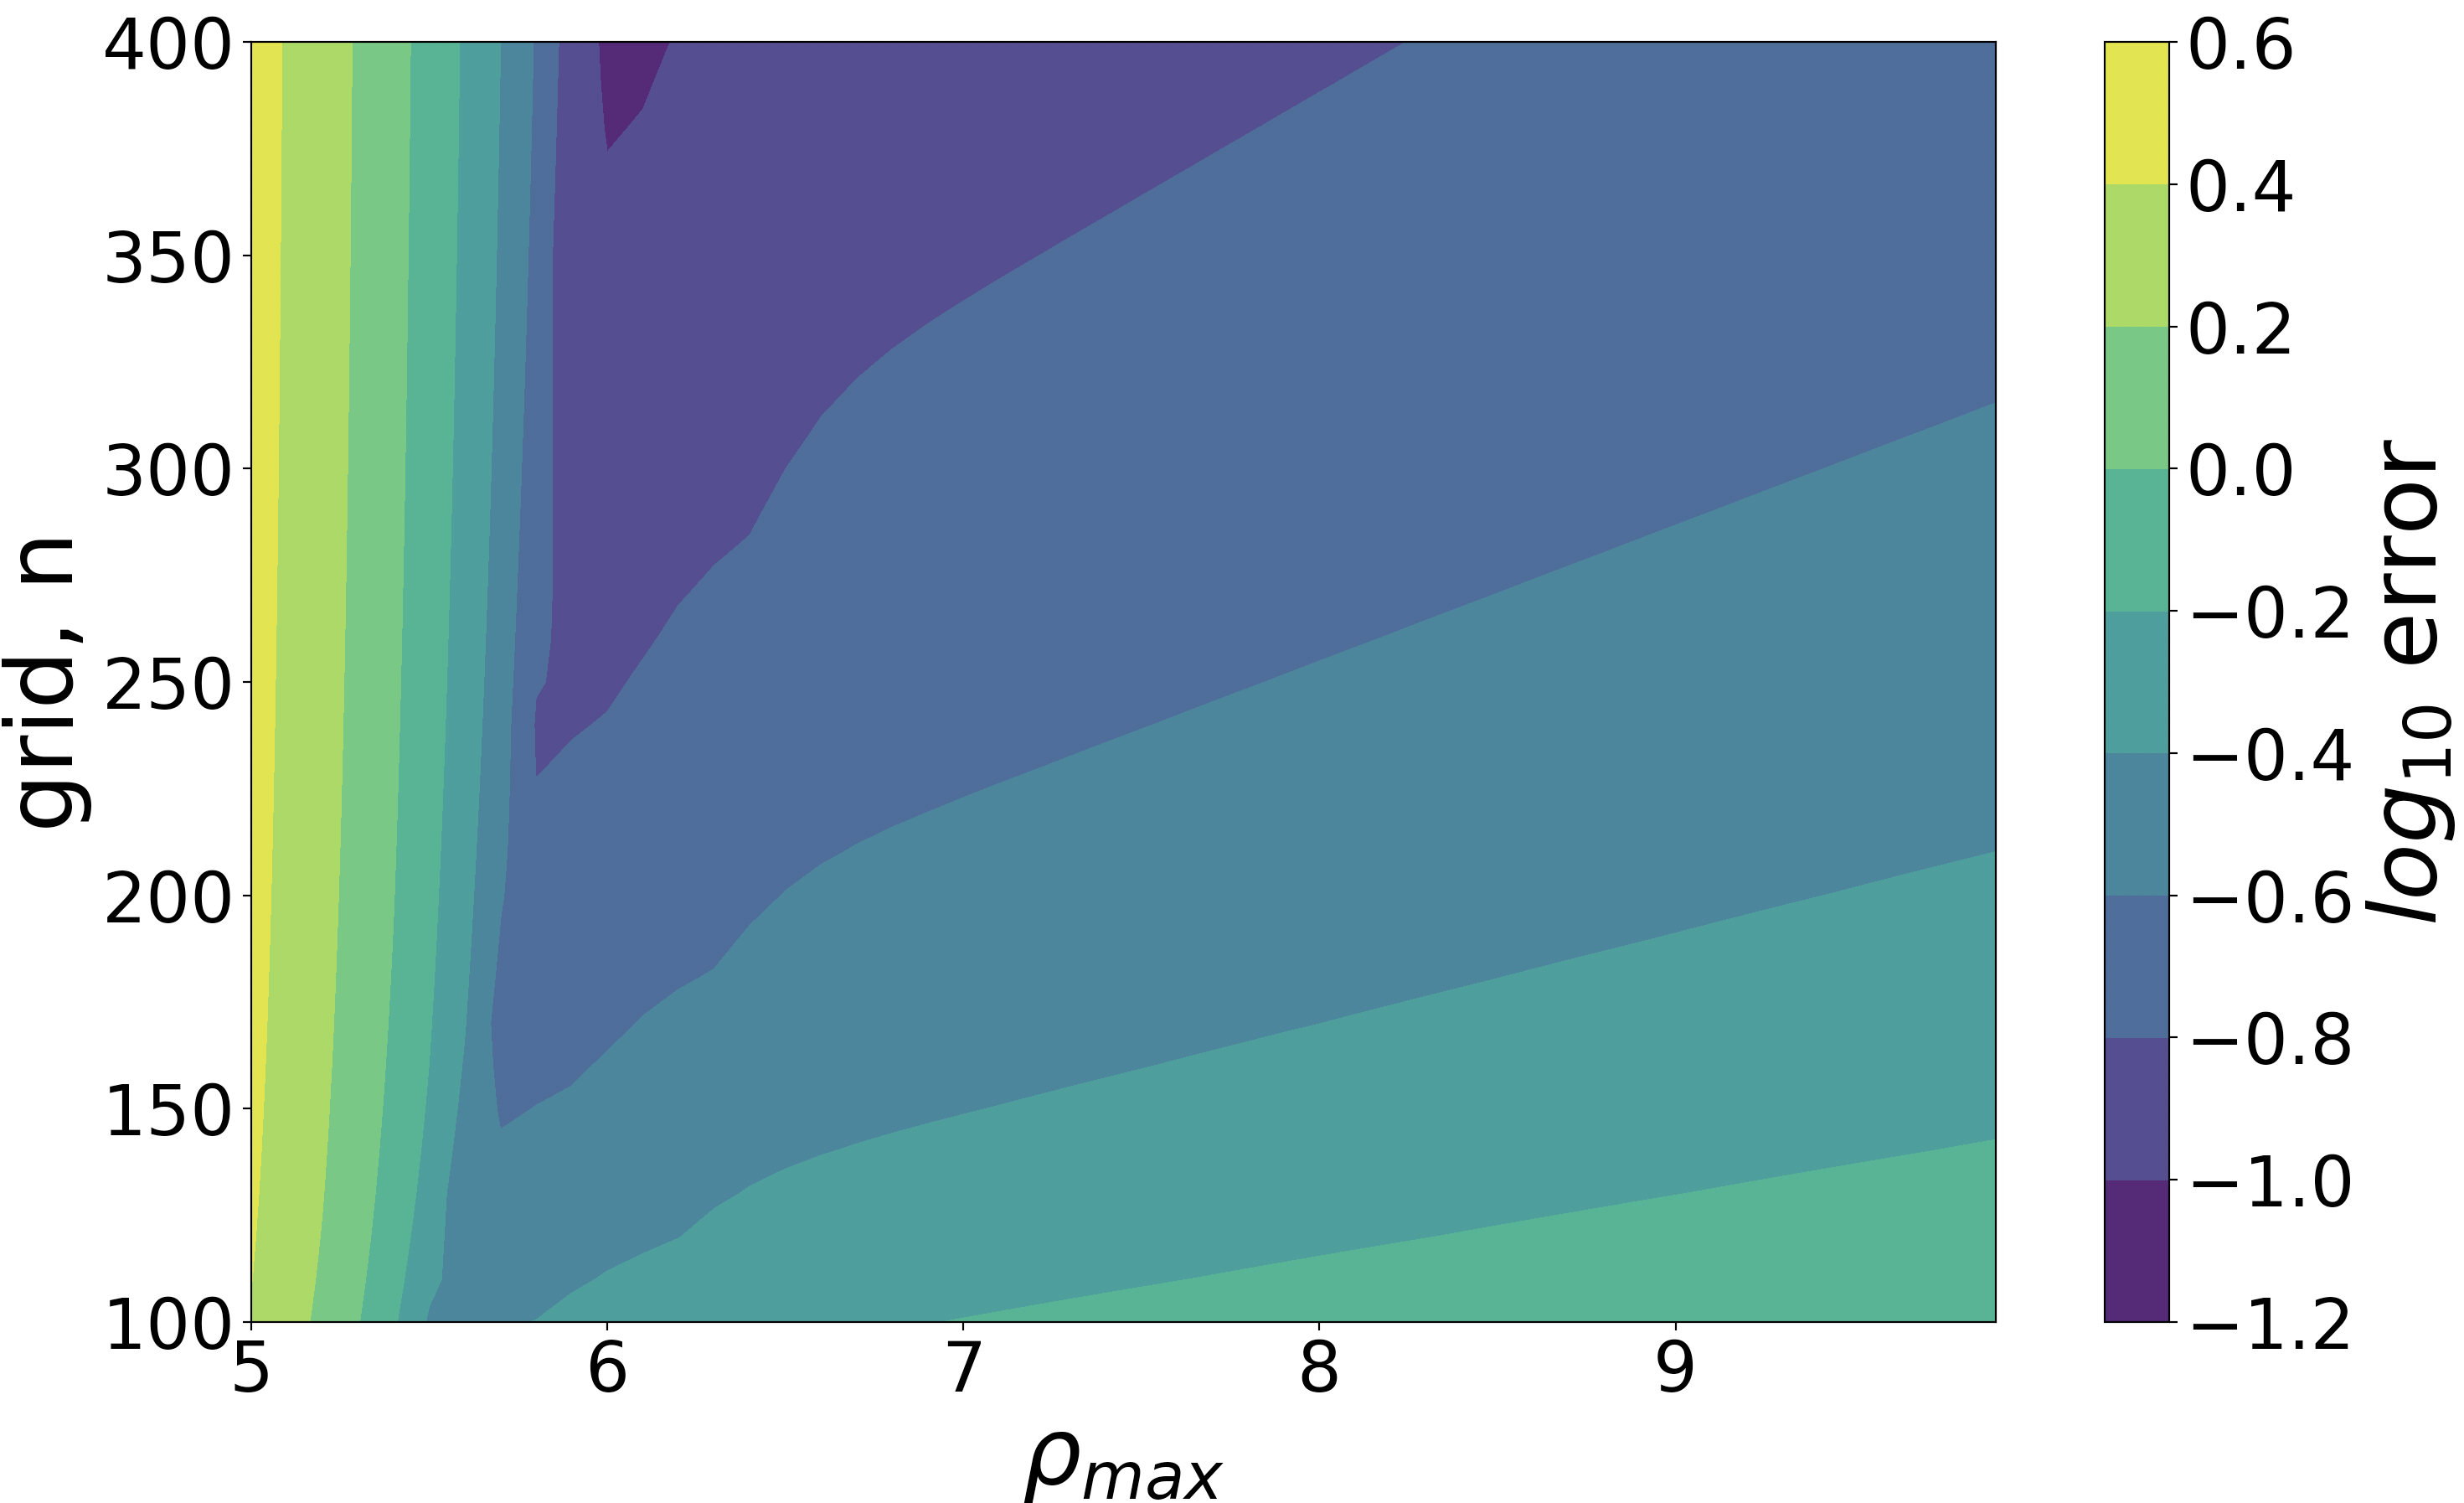
\includegraphics[scale=0.182]{max_error.png}
            \caption{A contour plot where the height (color) values are the maximum eigenvalue errors for a corresponding pair of $\rho_{\text{max}}$ and grid size values. The error values are converted to $\text{log}_{10}$ to better distinct differences between small error values. A clearly visible trend is that the error decreases as the grid size gets larger. A distinct area for the values $\rho_{\text{max}} \approx 6.1$ and $n\approx 400$ show the lowest maximum error.}
            \label{fig:max_error}
        \end{figure}{}
        
        Figure \ref{fig:min_error} displays the data in the same way as figure \ref{fig:max_error}, but with the minimum error instead of the maximum error of the eight first eigenvalues for each $\rho_{\text{max}}$ and grid size value. This view of the error reveals that there is no single pair of $\rho_{\text{max}}$ and grid size value that produce the lowest minimum error, as compared to the clearly distinct area in figure \ref{fig:max_error} where we can find the lowest maximum error. The minimum error stretch all the way down to $10^{-4}$ which is the limit we have aimed for.
        
        \begin{figure}[t]
            \centering
            %\hspace*{-1cm}
            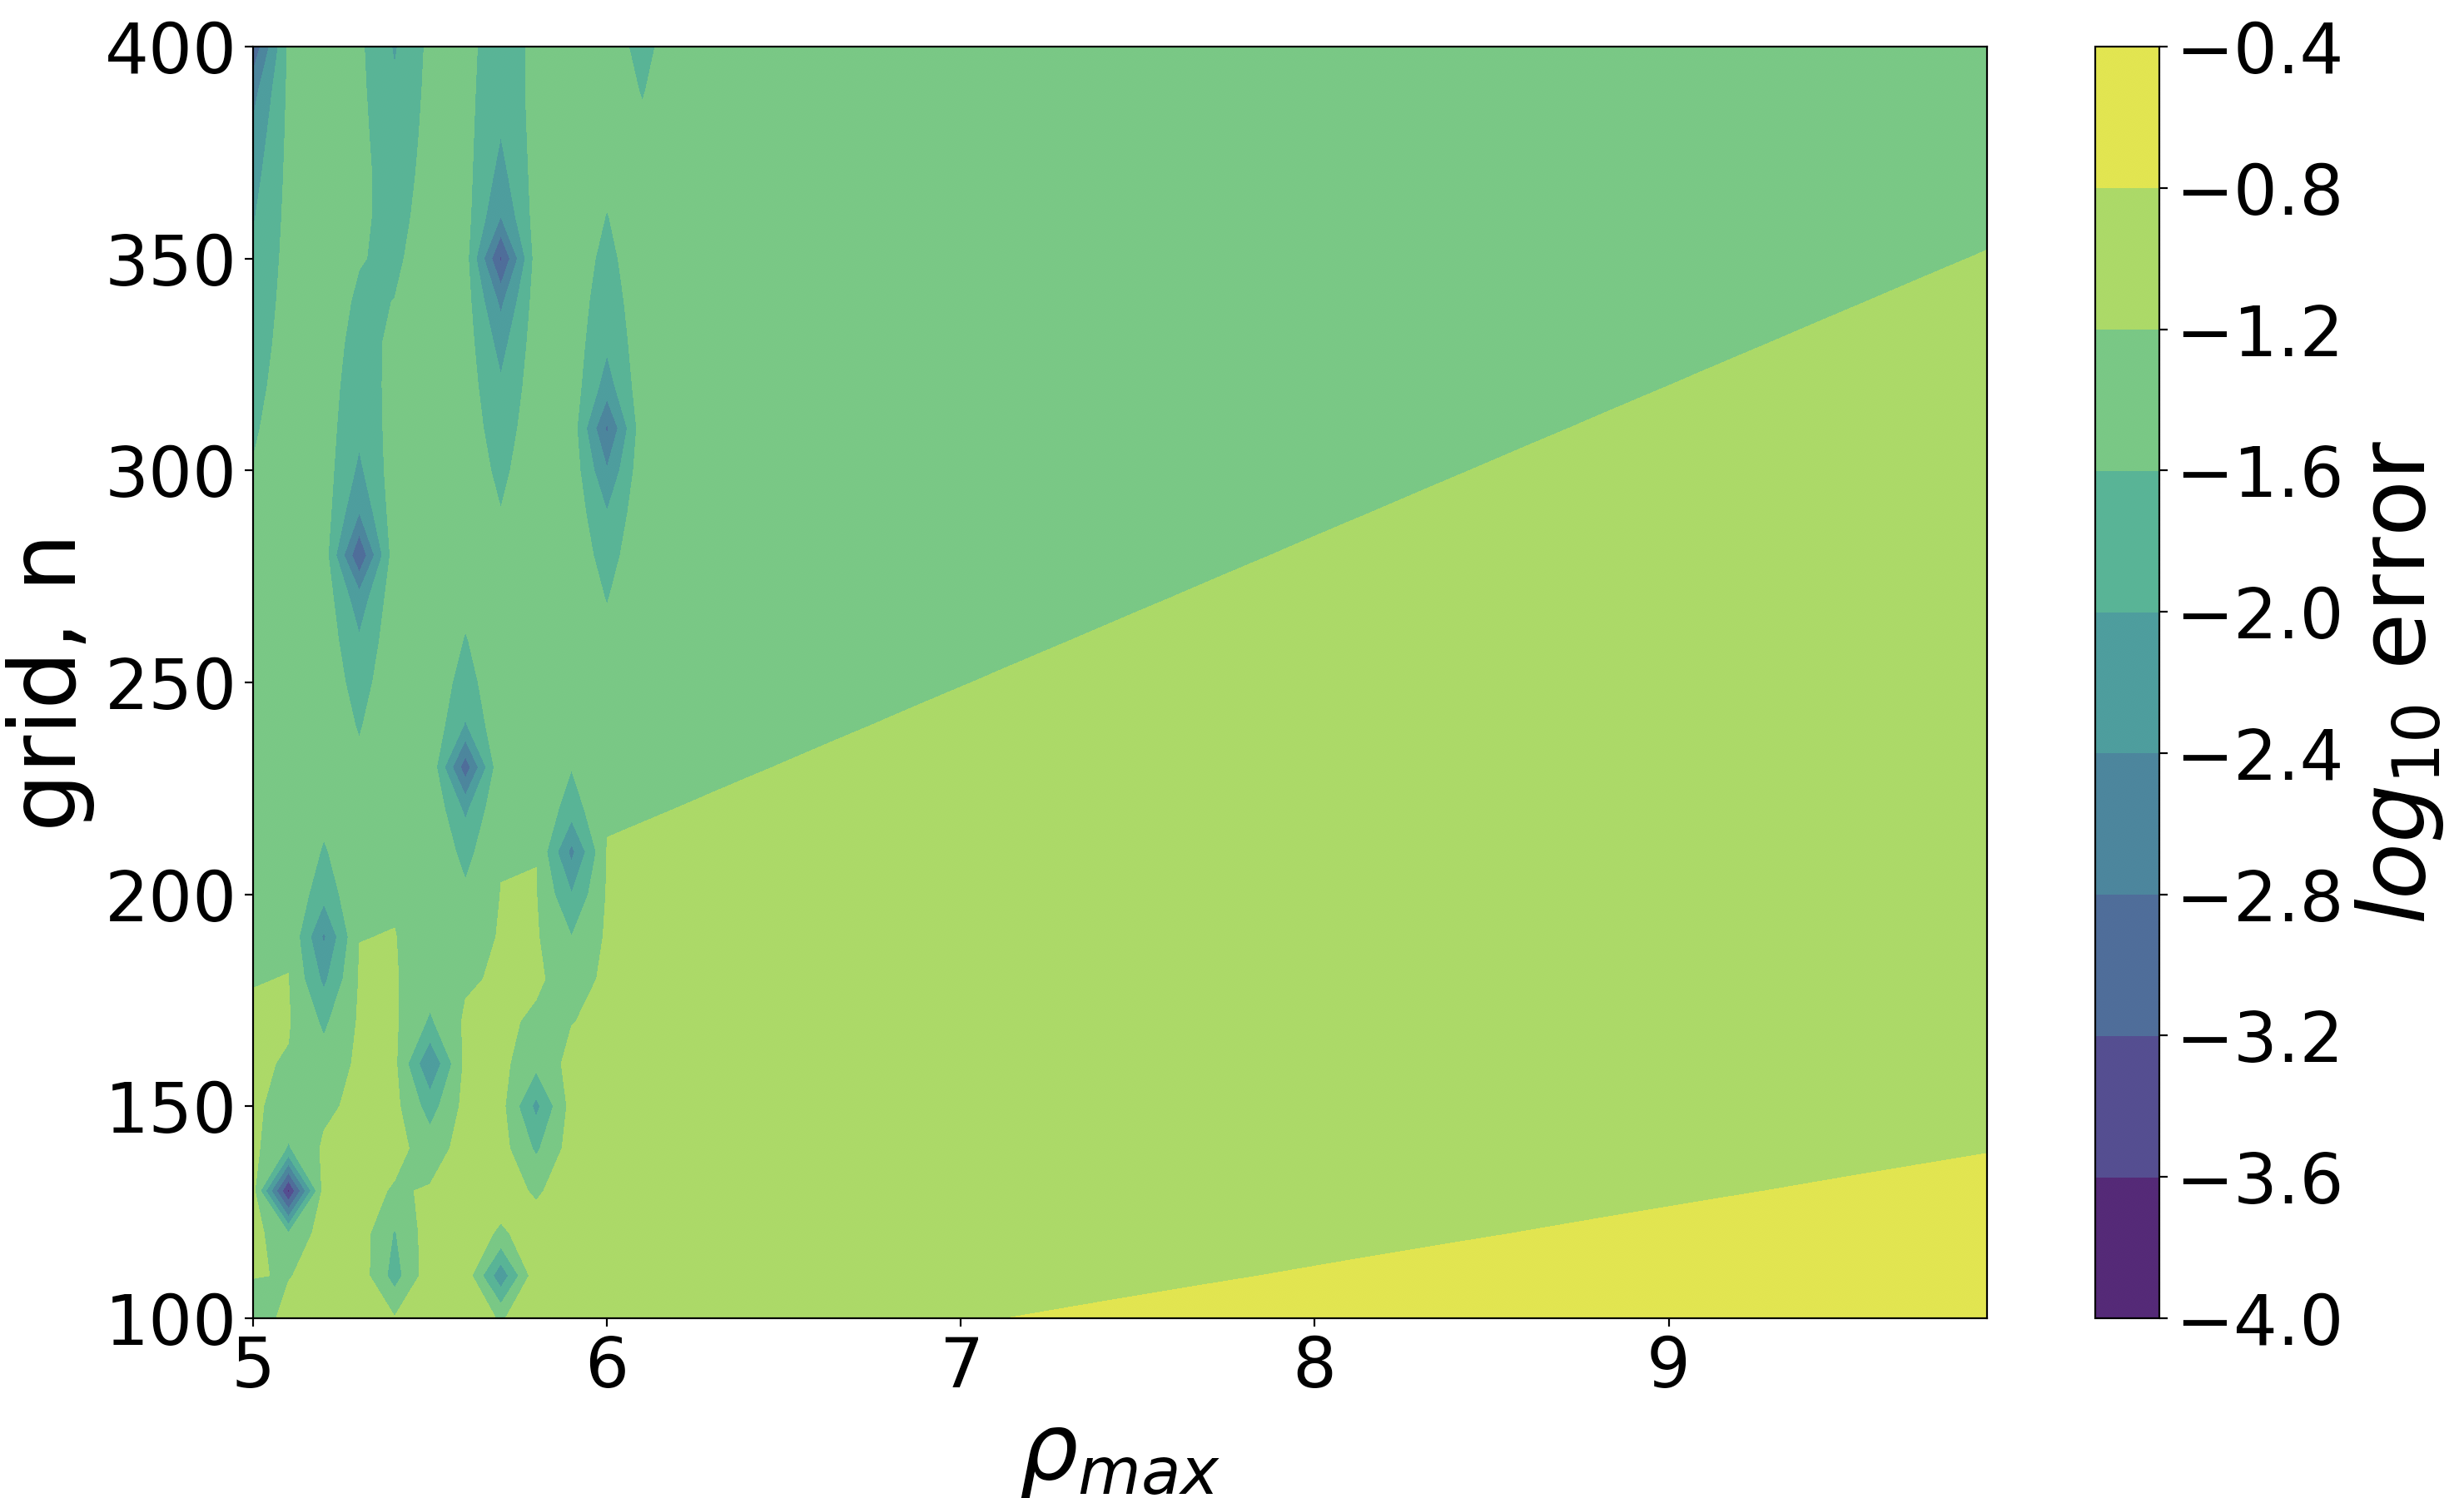
\includegraphics[scale=0.182]{min_error.png}
            \caption{A contour plot where the height (color) values are the minimum eigenvalue errors for a corresponding pair of $\rho_{\text{max}}$ and grid size values. The error values are converted to $\text{log}_{10}$ to better distinct differences between small error values. It comes to light that there is no concentrated area where the minimum errors are located.}
            \label{fig:min_error}
        \end{figure}{}
        
        Another view of the contour plot in figure \ref{fig:max_error} is displayed in figure \ref{fig:error_vs_rhomax}. Here we see three graphs, each representing the maximum error of eight calculated eigenvalues for each $\rho_{\text{max}}$. The three graphs are for $n = 100$, $n = 250$ and $n = 400$.
        
        We can clearly see that the highest errors are for the lowest values of $\rho_{\text{max}}$. For higher grid point values, $n$, the error starts off as higher, but at $\rho_{\text{max}} \approx 5.7$ the higher grid point values yield lower errors. We notice that with high grid point values, as we see with $n = 250, n = 400$, the error settles at around $\rho_{\text{max}} \approx 6$, and barely rises after that.
        
        
        \begin{figure}[t]
            \centering
            %\hspace*{-1cm}
            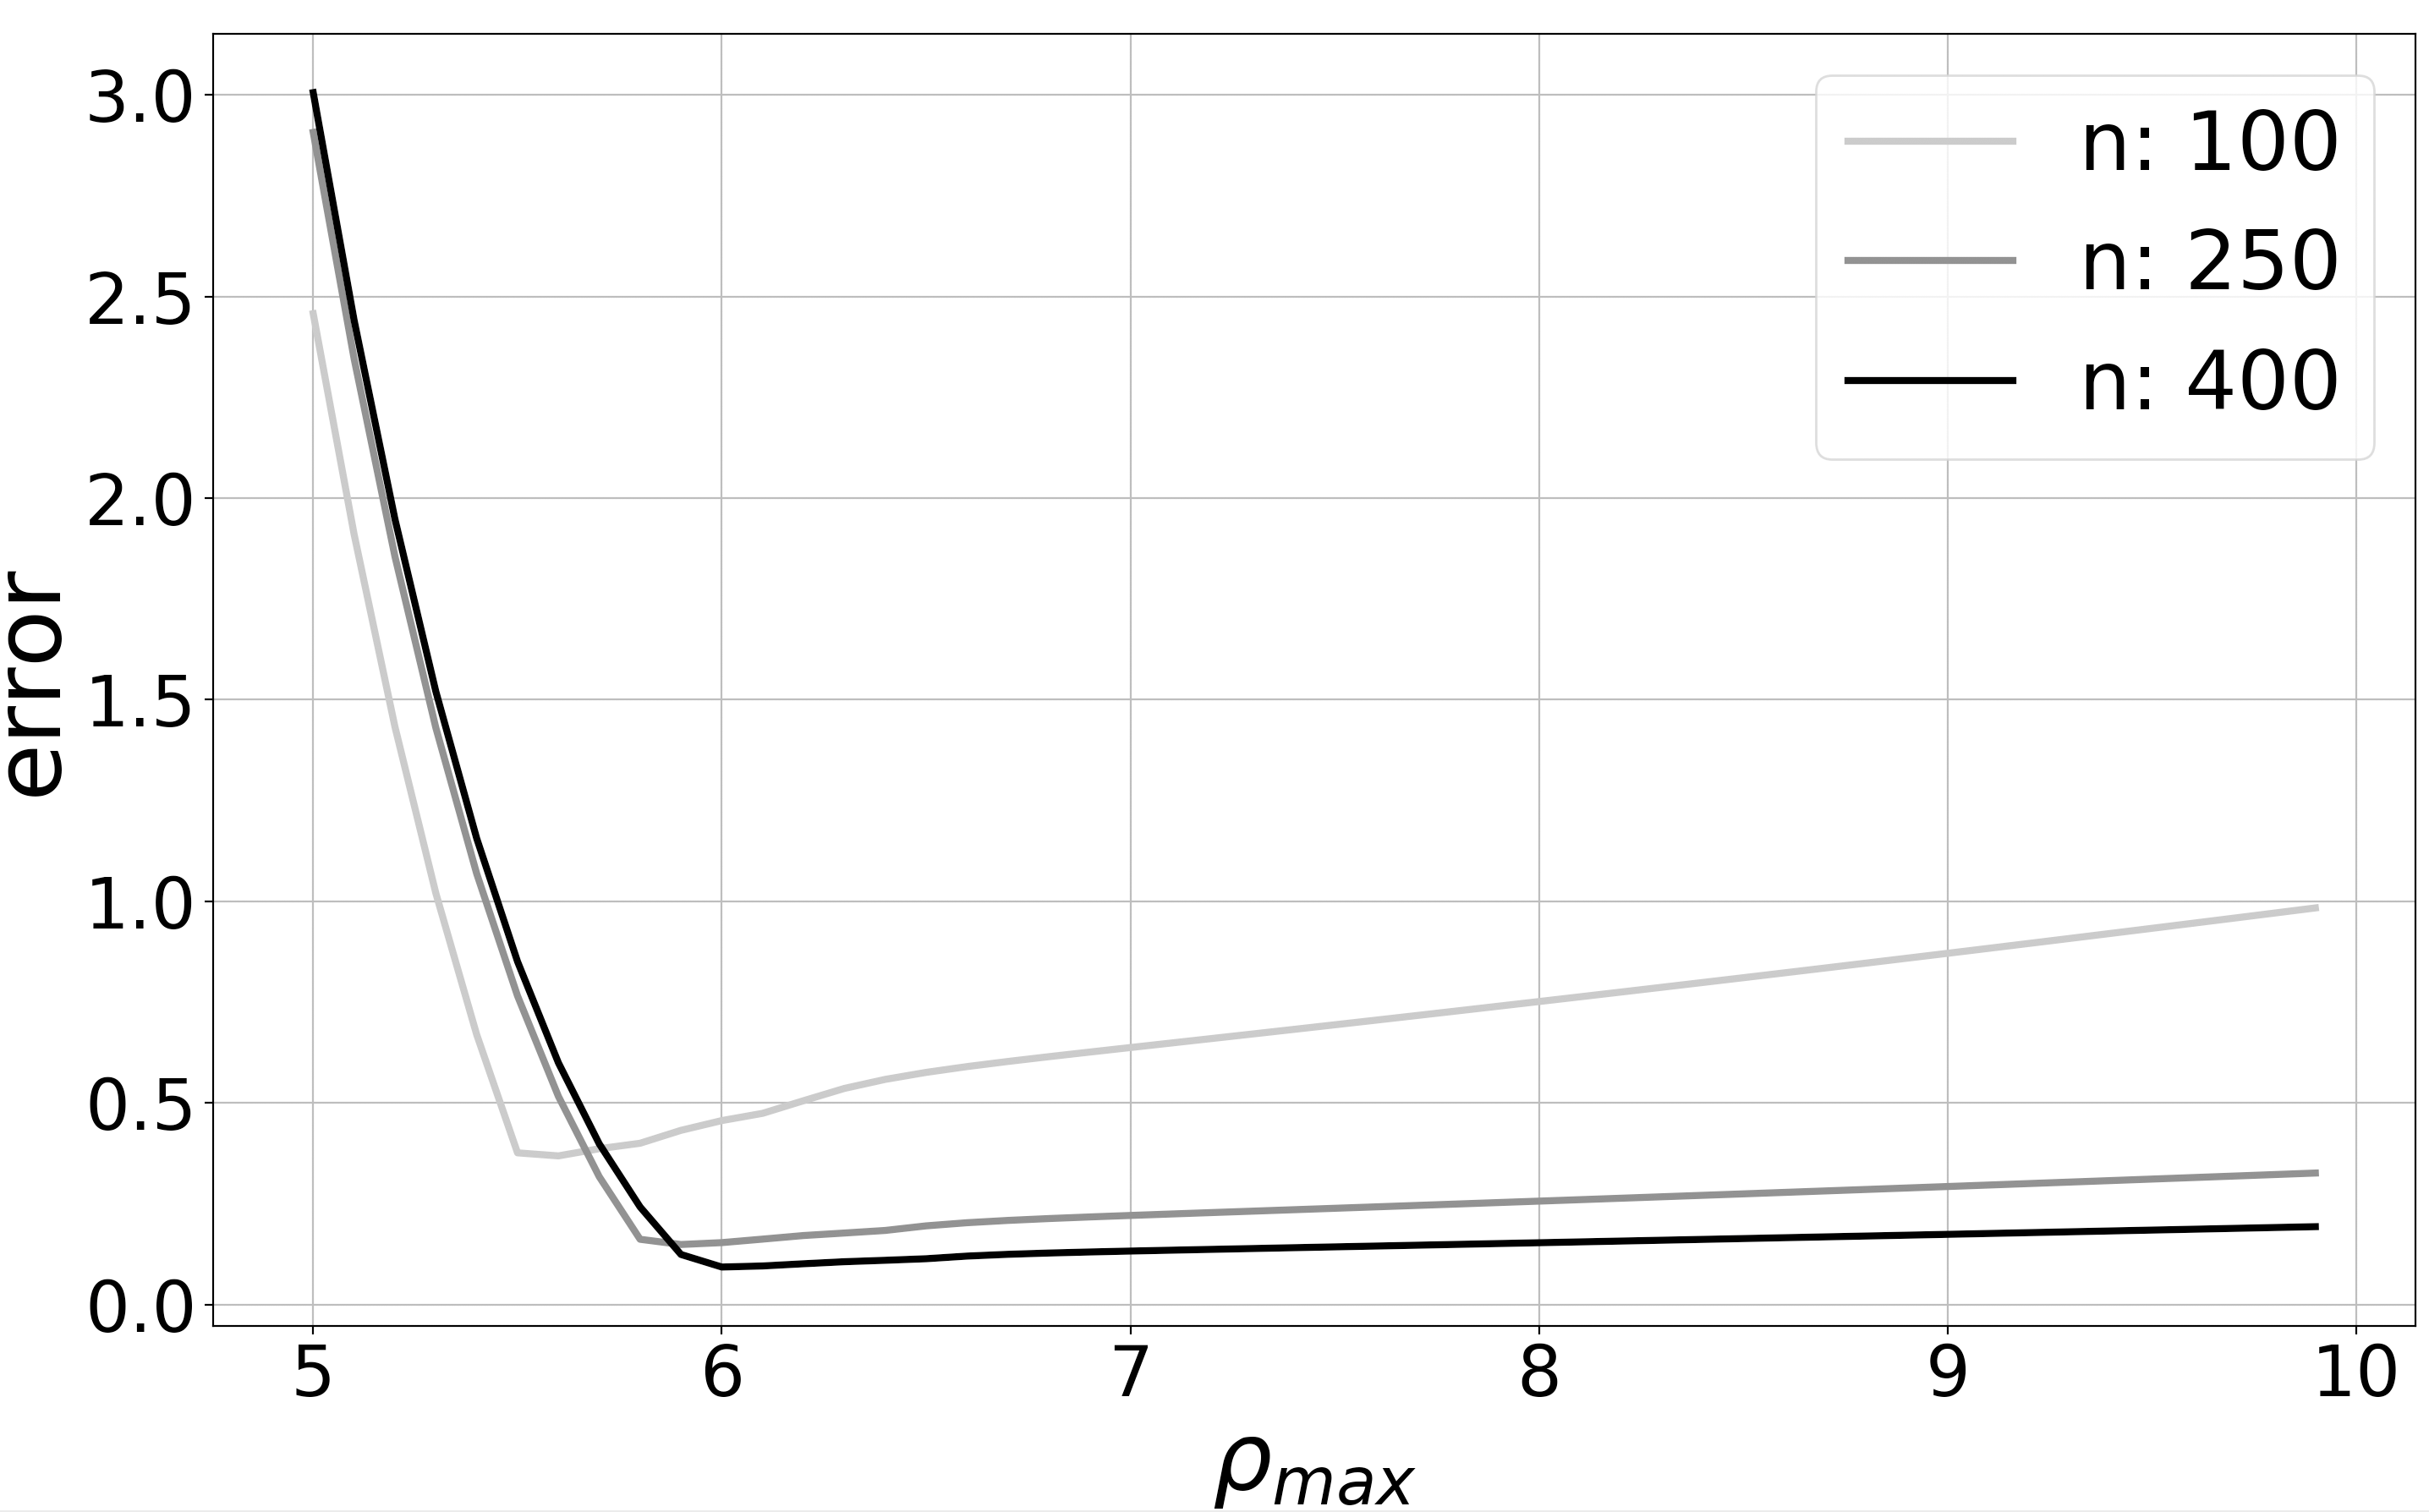
\includegraphics[scale=0.16]{error_vs_rhomax.png}
            \caption{The plot shows graphs for the maximum error of eight eigenvalues calculated for each $\rho_{\text{max}}$. The three different graphs are for $n = 100$, $n = 250$ and $n = 400$.}
            \label{fig:error_vs_rhomax}
        \end{figure}{}
        
        In figure \ref{fig:error_vs_rhomax_ground_state} we can see the error for the first eigenvalue - the eigenvalue of the ground state - as a function of $\rho_{\text{max}}$. The trend we can see here is quite different from the maximum error of the eight first eigenvalues, as displayed in figure \ref{fig:error_vs_rhomax}. A larger grid size does yield lower errors, but the lowest $\rho_{\text{max}}$ is the value which gives the lowest error, and if we do a bit of a mental extrapolation, it seems that even lower values of $\rho_{\text{max}}$ will give better results.
        
        
        
        \begin{figure}[t]
            \centering
            %\hspace*{-1cm}
            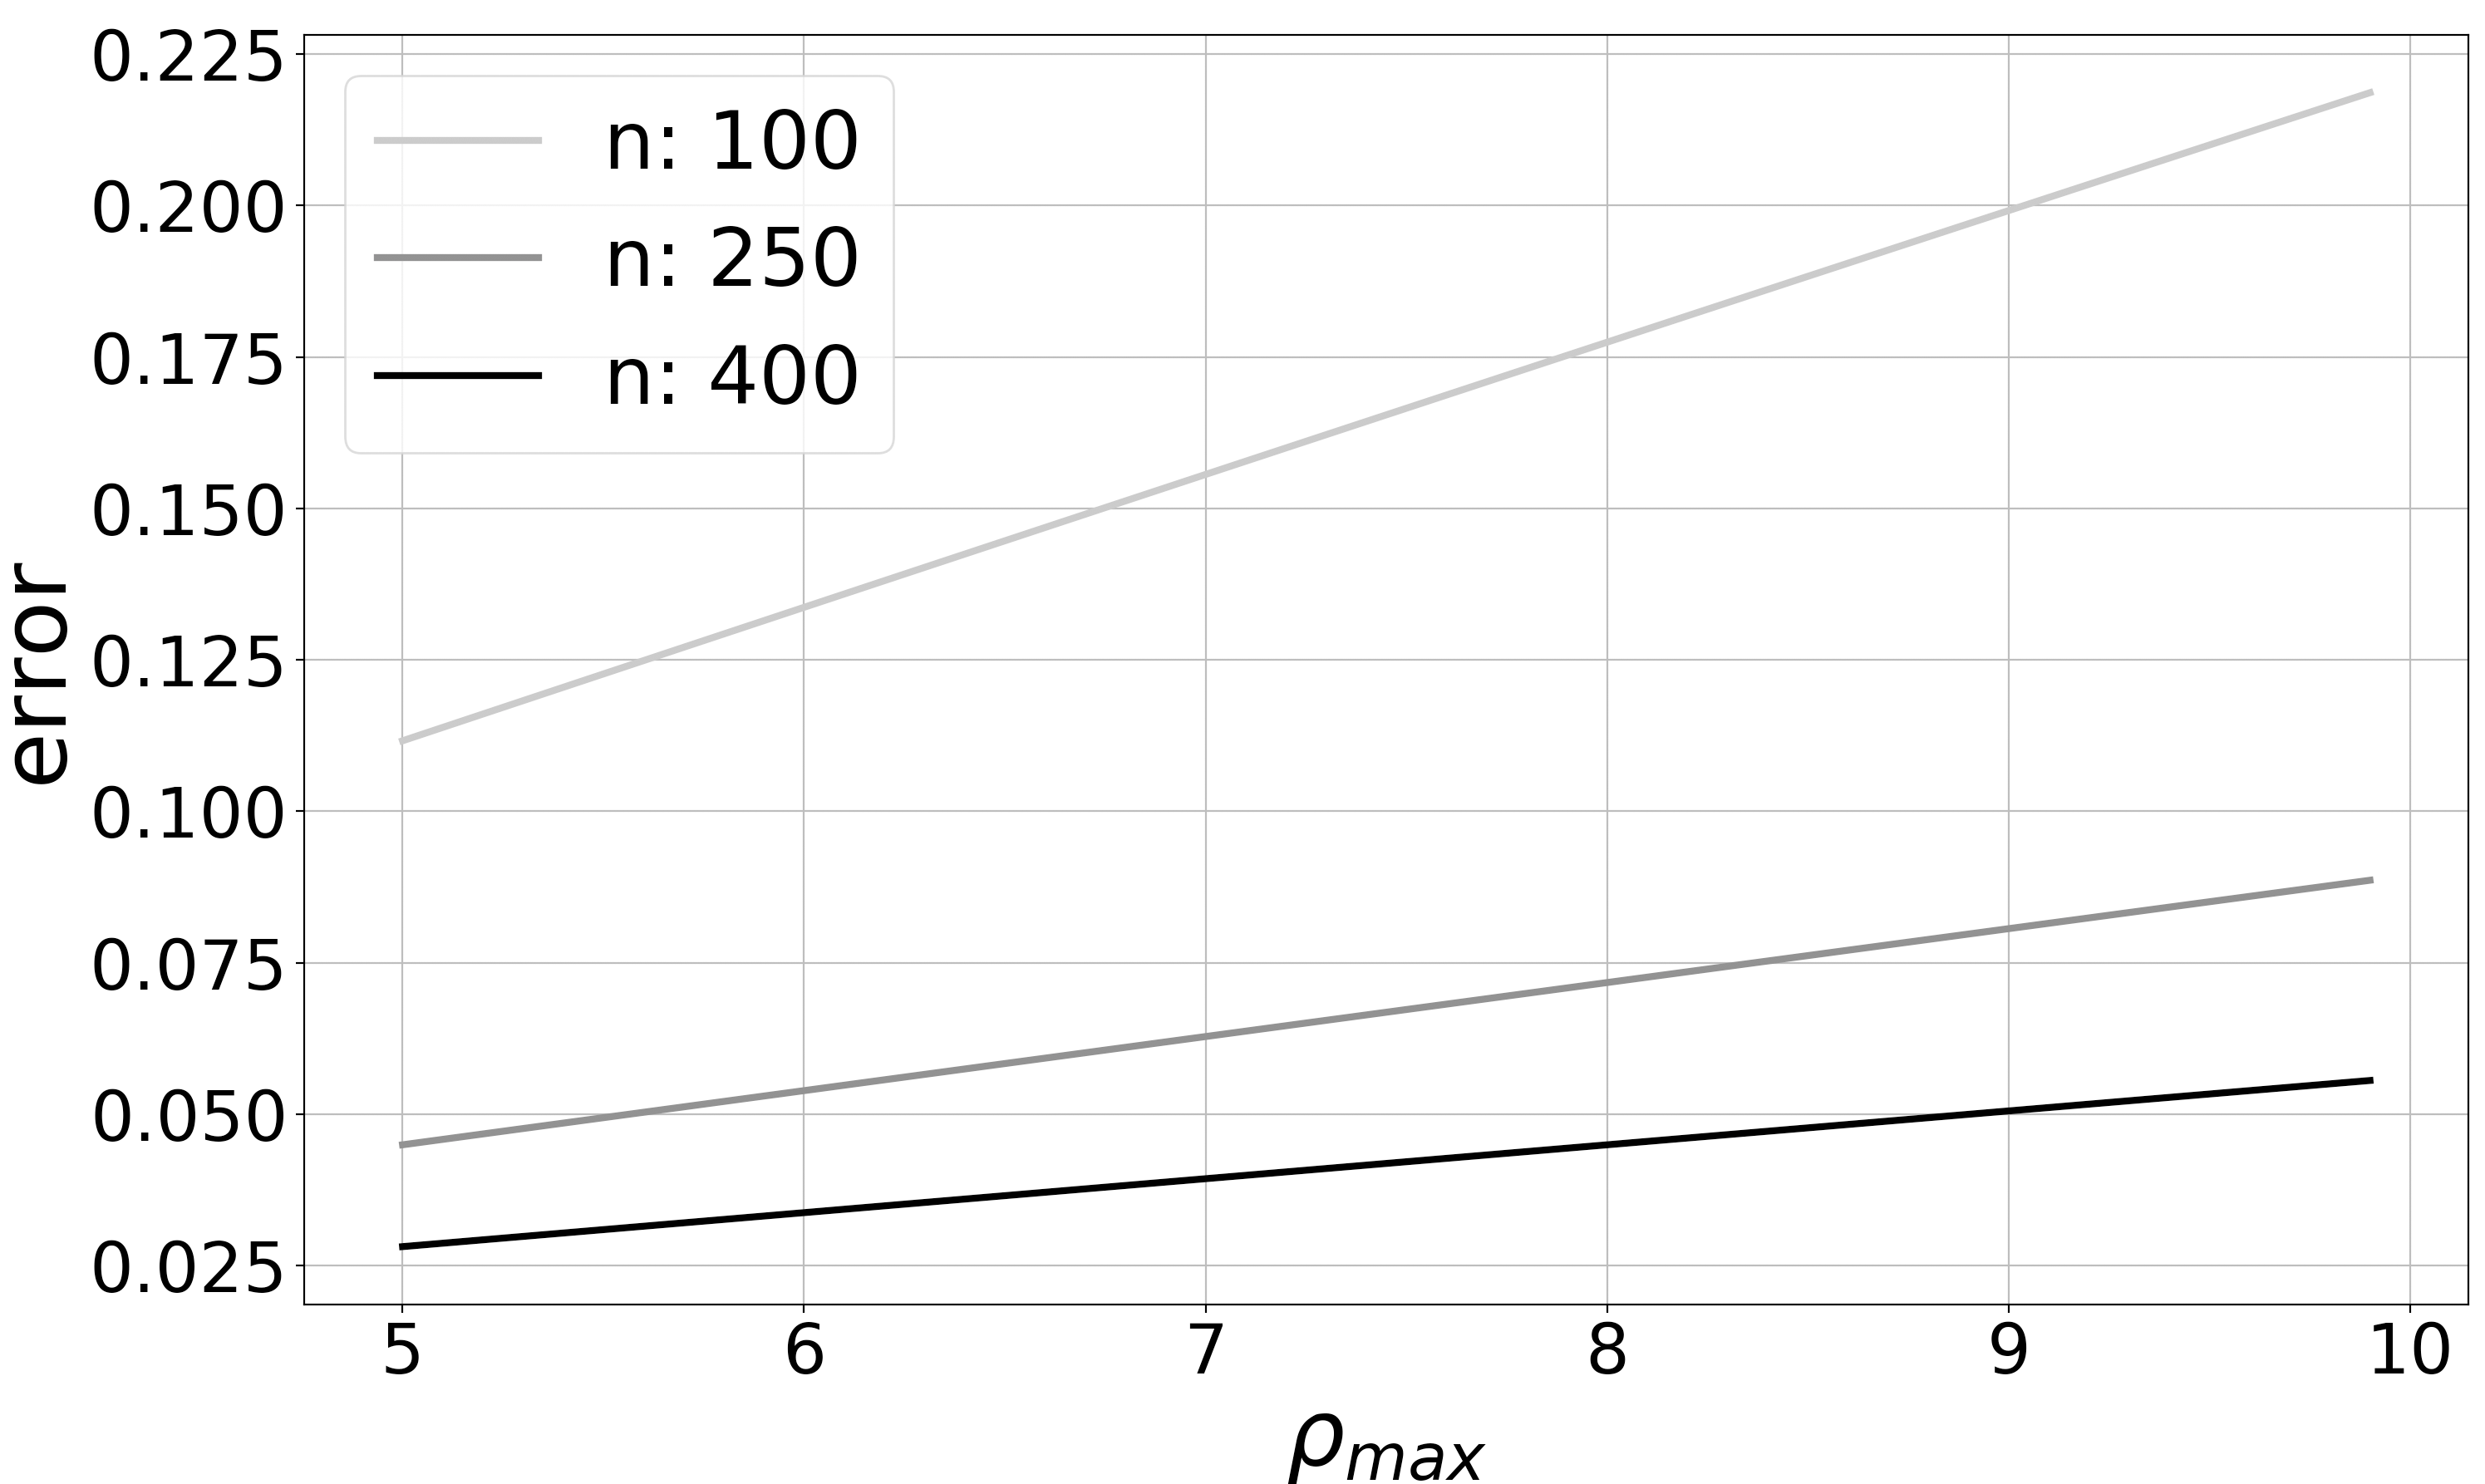
\includegraphics[scale=0.16]{error_vs_rhomax_ground_state.png}
            \caption{The plot shows graphs for the ground state eigenvalue for each $\rho_{\text{max}}$. The three different graphs are for $n = 100$, $n = 250$ and $n = 400$.}
            \label{fig:error_vs_rhomax_ground_state}
        \end{figure}{}
        
    \subsection{\textbf{Two electron system}}
        
        Figure \ref{fig:w_005} shows the radial wavefunction for $\omega_r = 0.05$ with the calculated and analytical solution plotted. We can see from the figure that the overlap is good.
        A study of the accompanying eigenvalue shows that it is $\lambda_c = 0.3499996012$. With the analytical value $\lambda_a = 0.35$ we get a calculation error of $\approx 3.99 \cdot 10^{-7}$.
        
        Similarly, figure \ref{fig:w_025} shows the radial wavefunction for $\omega_r = 0.05$ with the calculated and analytical solution plotted. There is a good overlap here as well.
        The accompanying eigenvalue is $\lambda_c = 0.3499996012$. With the analytical value $\lambda_a = 0.35$ we get a calculation error of $\approx 3.99 \cdot 10^{-7}$.
        
        \begin{figure}[t]
            \centering
            %\hspace*{-1cm}
            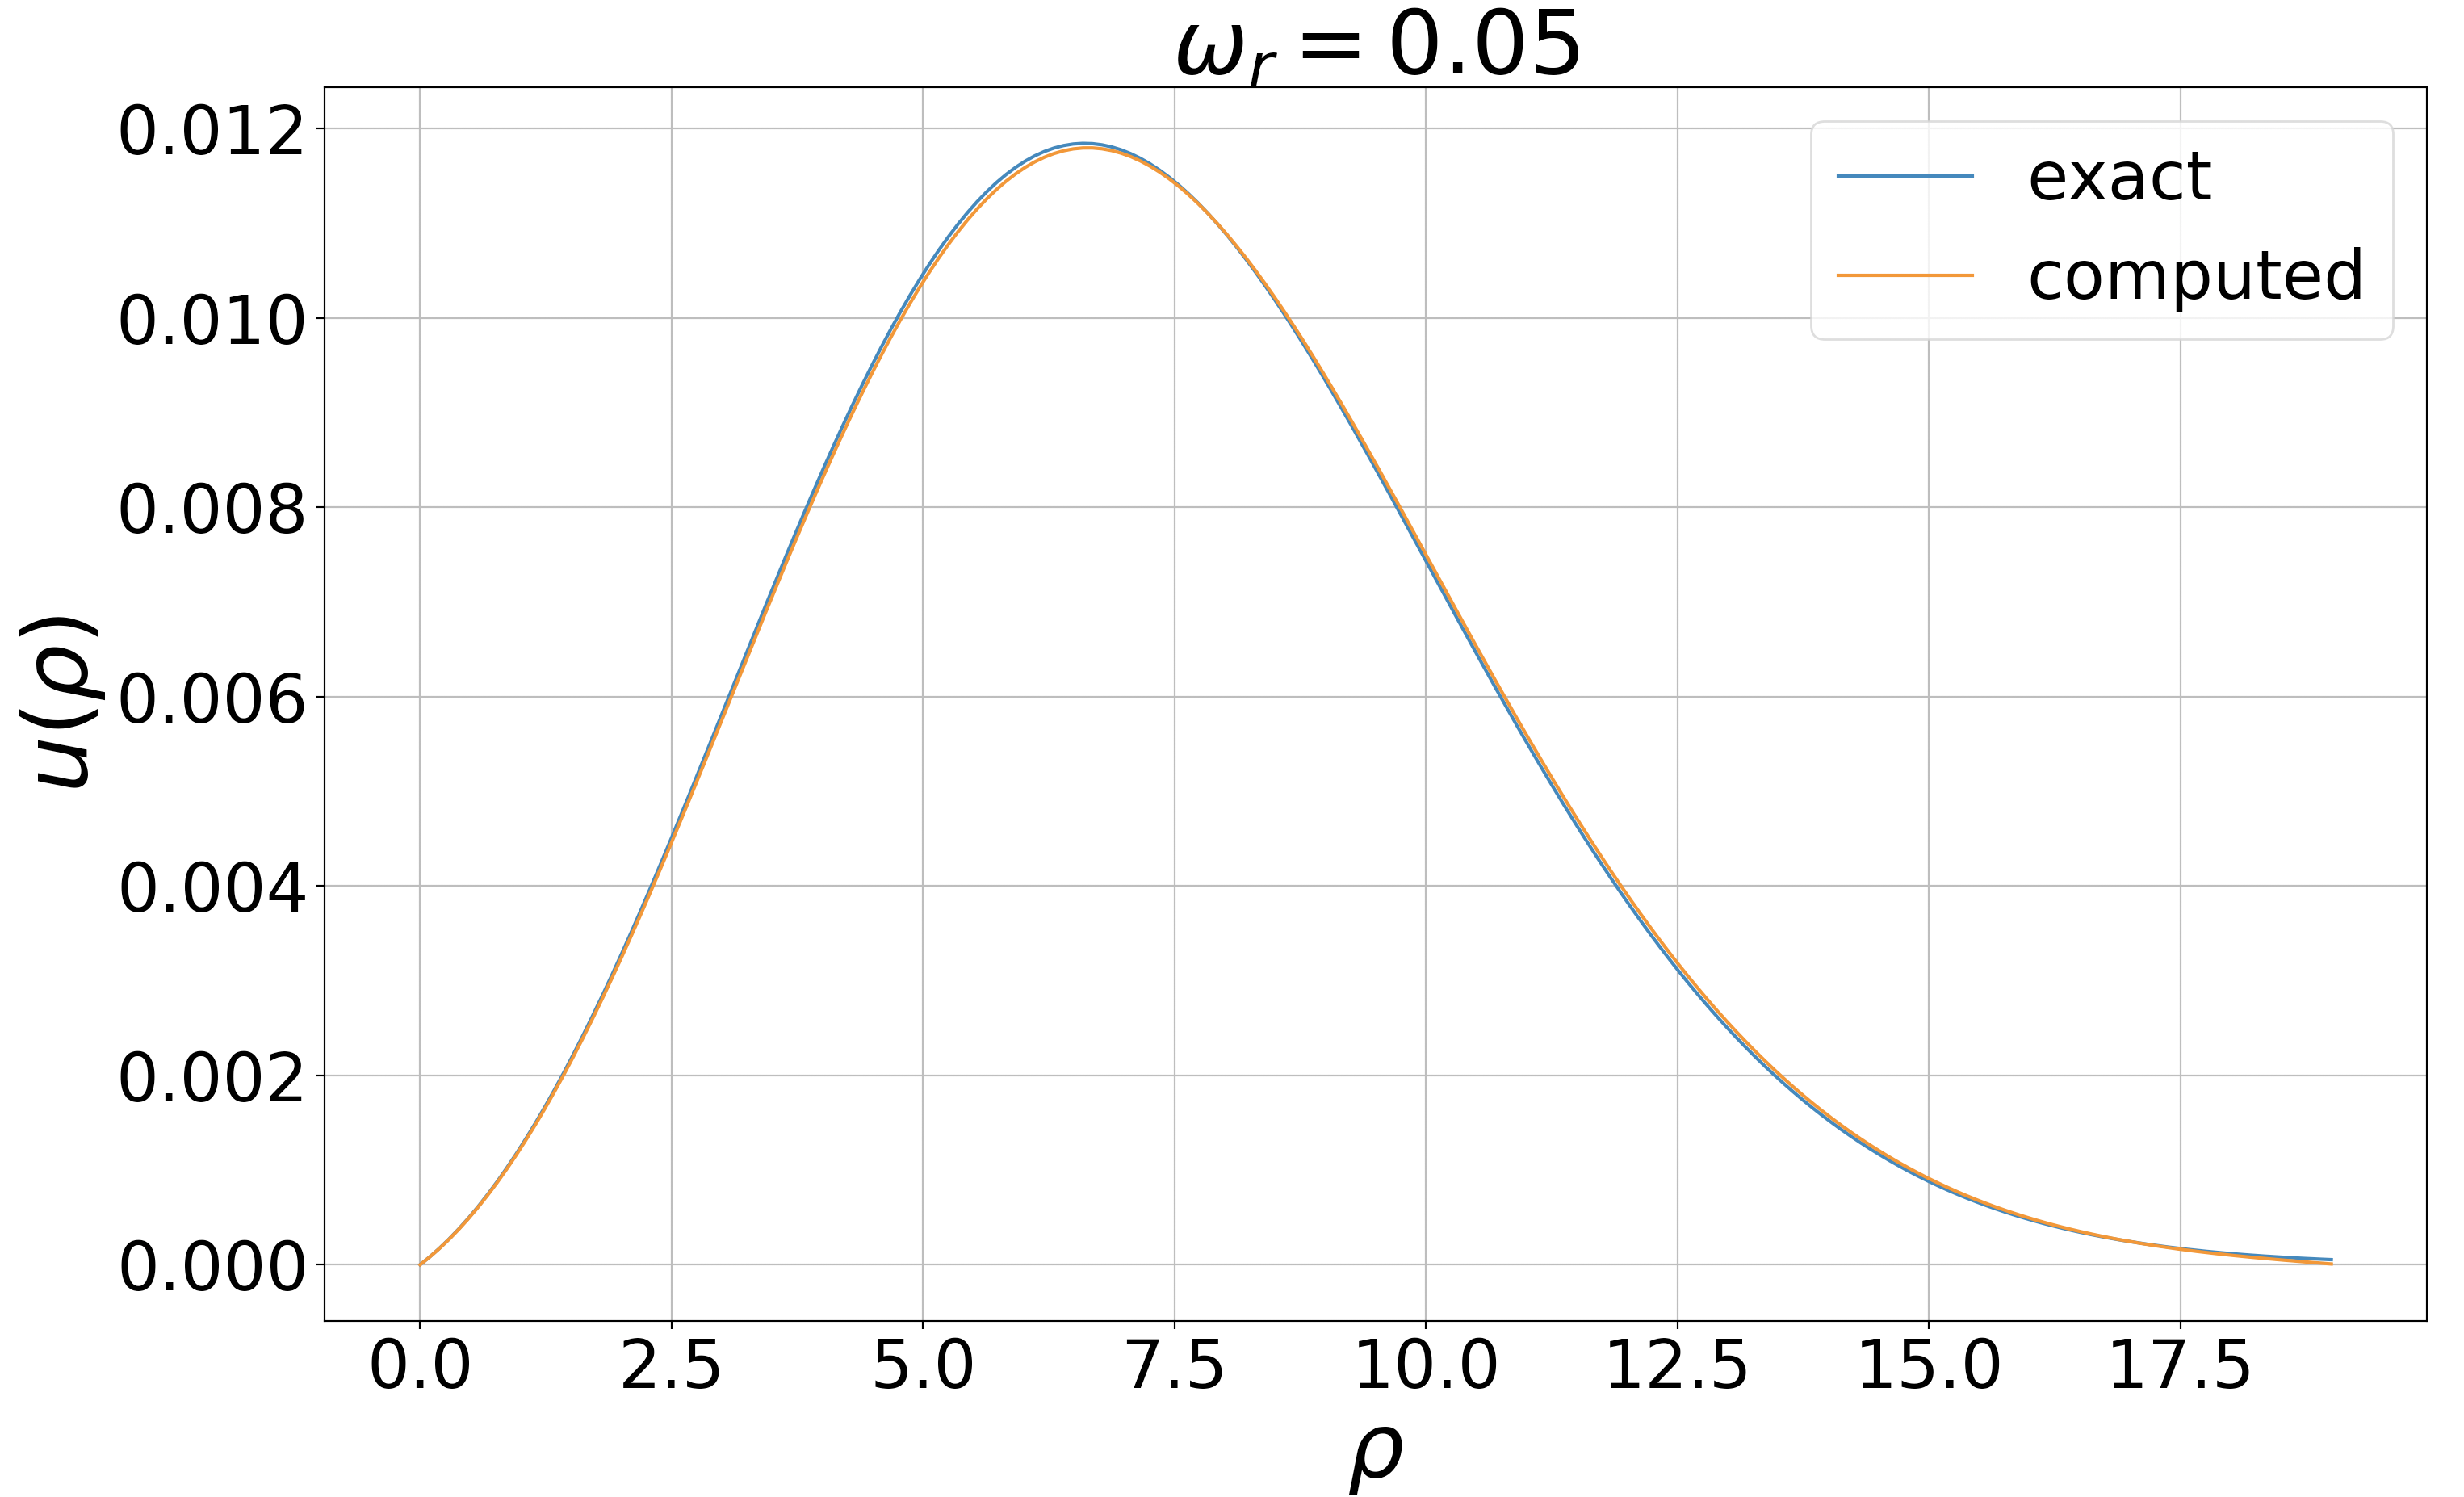
\includegraphics[scale=0.16]{w_005.png}
            \caption{The radial wavefunction for harmonic oscillator frequency $\omega_r = 0.05$. The analytical and computed solutions are plotted and the graphs have a good overlap. The calculated eigenvalue was found to be $\lambda_c = 1.24999382$. The analytical value is $\lambda_a = 1.25$ which yields a calculation error of $\approx 6.18 \cdot 10^{-6}$.}
            \label{fig:w_005}
        \end{figure}{}
        
        
        \begin{figure}[t]
            \centering
            %\hspace*{-1cm}
            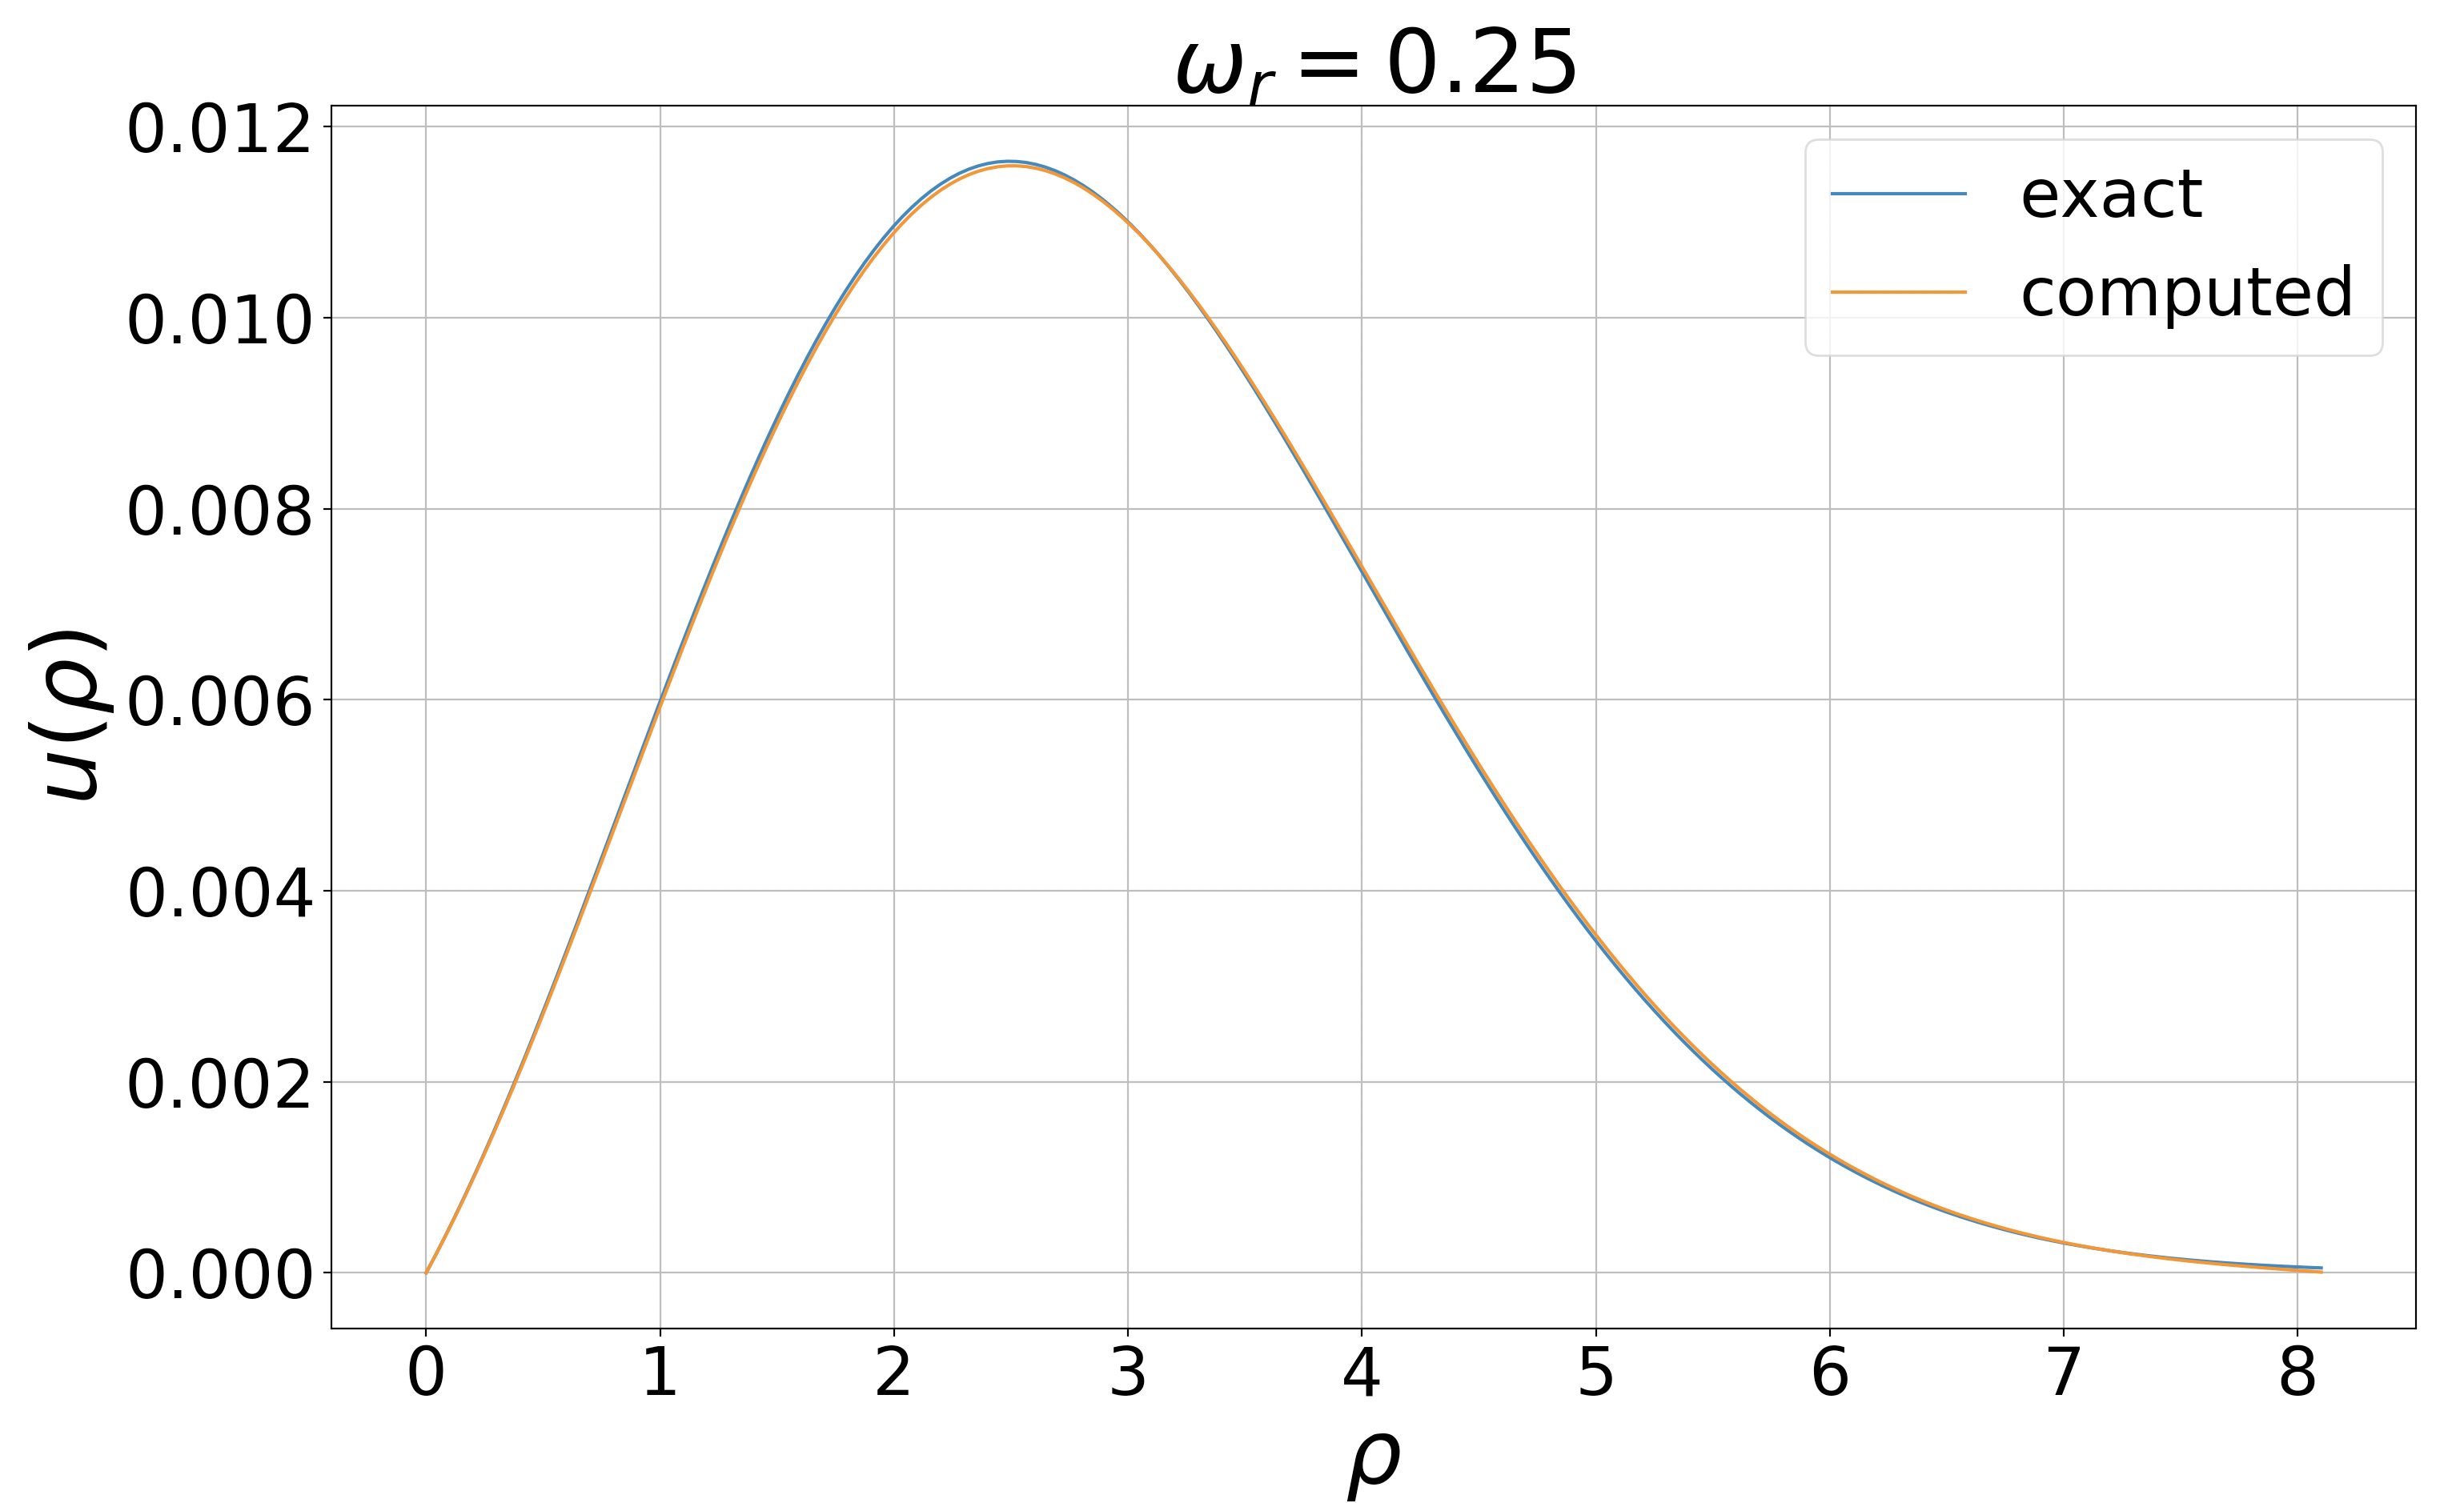
\includegraphics[scale=0.16]{w_025.png}
            \caption{The radial wavefunction for harmonic oscillator frequency $\omega_r = 0.25$. The analytical and computed solutions are plotted and the graphs have a good overlap. The calculated eigenvalue was found to be $\lambda_c = 1.24999382$. The analytical value is $\lambda_a = 1.25$ which yields a calculation error of $\approx 6.18 \cdot 10^{-6}$.}
            \label{fig:w_025}
        \end{figure}{}
        
        Figure \ref{fig:all_waves} show the radial part of the wavefunction for harmonic oscillator frequencies $\omega_r = [0.01, 0.05, 0.25, 0.5, 1, 5]$. As we can see, the graphs widens for low frequencies and tightens for high frequencies. Due to grid size limitations, the graphs are a bit off in the sense that the wider graphs should be lower than the shallow ones. We simply did not have time to run all the calculations for higher grid values than $n = 200$. 
        
        \begin{figure}[t]
            \centering
            %\hspace*{-1cm}
            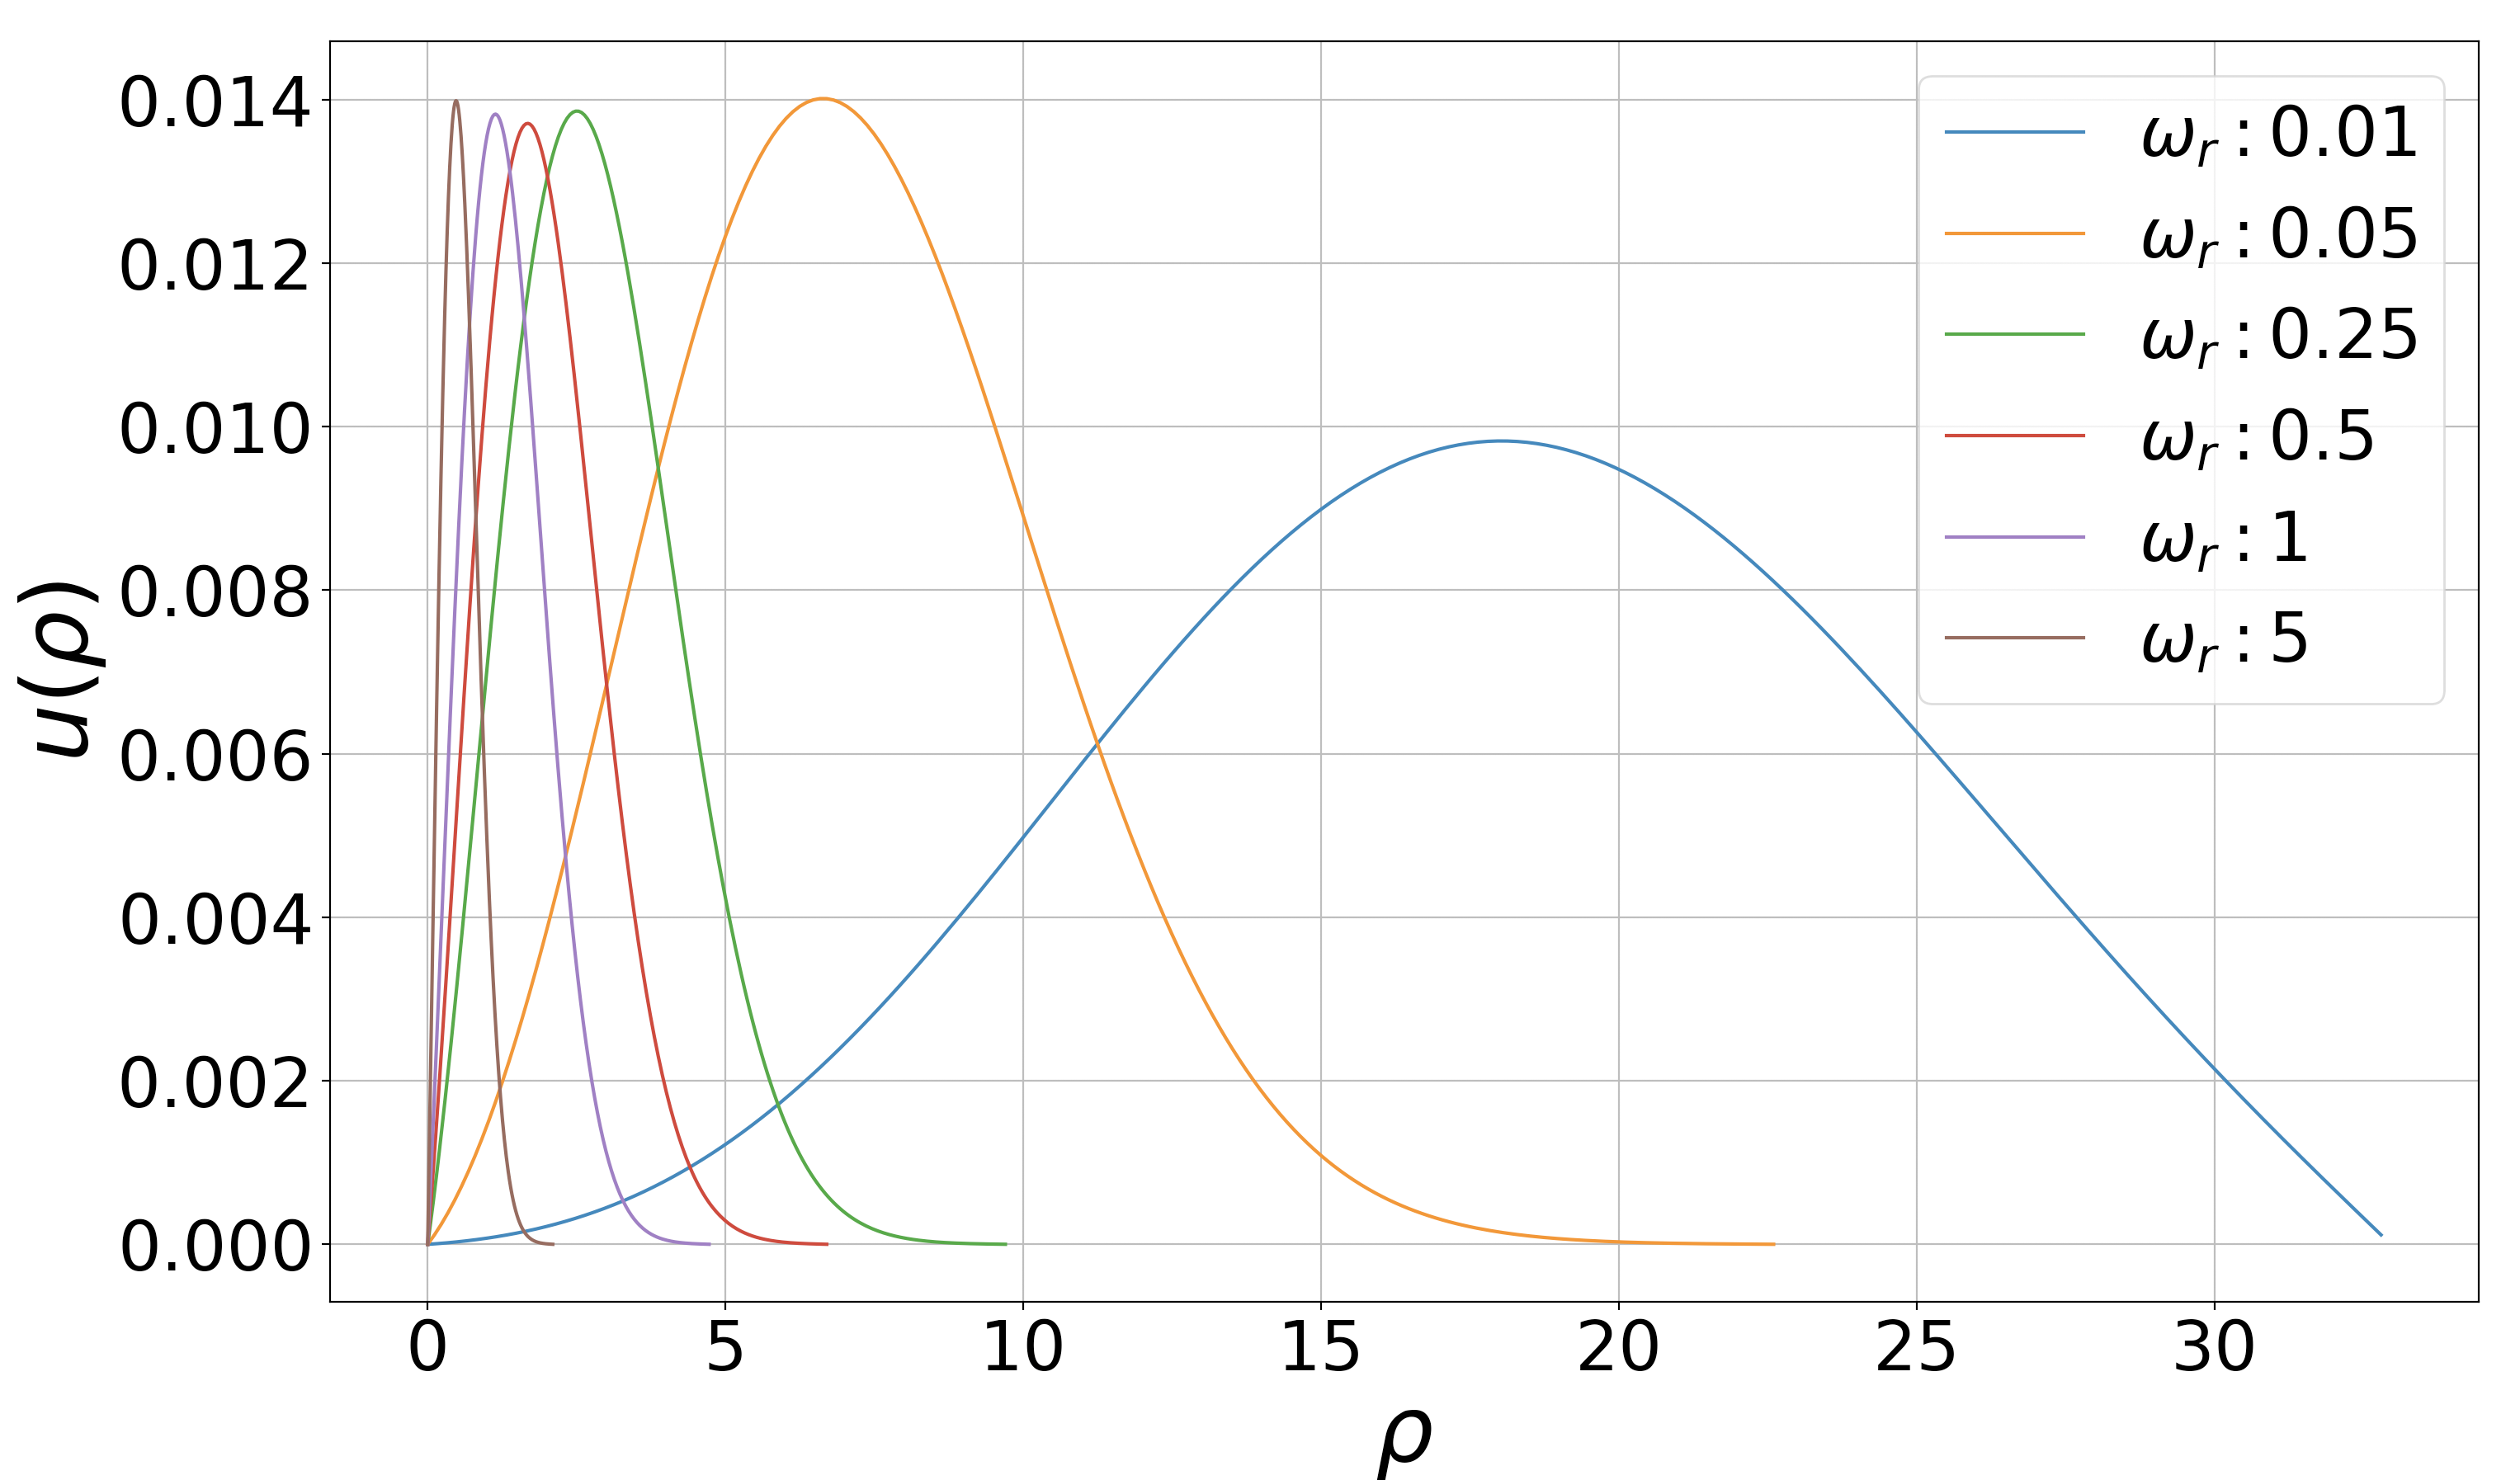
\includegraphics[scale=0.16]{all_waves.png}
            \caption{The figure shows the radial part of the wavefunction for harmonic oscillator frequencies $\omega_r = [0.01, 0.05, 0.25, 0.5, 1, 5]$.}
            \label{fig:all_waves}
        \end{figure}{}
        
    
    

%%%%%%%%%%%%%%%%%%%%%%%%%%%%%%%%%%%%
%%%%%%%%%%%%%%%%%%%%%%%%%%%%%%%%%%%%
\section{\textbf{Conclusion}}
%%%%%%%%%%%%%%%%%%%%%%%%%%%%%%%%%%%%
%%%%%%%%%%%%%%%%%%%%%%%%%%%%%%%%%%%%
    By using discretization of the double derivative and representing it as a matrix, we have been able to use some of the powerful tools of linear algebra to solve a quantum mechanical system. By identifying the electron energy levels as the eigenvalues of the matrix and the electron states as the corresponding eigenvectors, we have used Jacobis eigenvalue algorithm to extract the information and given an estimation of its numerical precision.
    
    During this study, it came to light that the best grid and $\rho_{\text{max}}$ values for finding the lowest maximum eigenvalue error for the eight first eigenvalues for the single electron system are $\rho_{\text{max}} \approx 6.1$ and $n = 400$. It is seen in figure \ref{fig:max_error}. We also saw that the lowest minimum eigenvalue error for the same system is not concentrated in a single area, but rather spread out over a number of grid and $\rho_{\text{max}}$ value pairs. This is seen in figure \ref{fig:min_error}.
    
    A further analysis showed that the same system yields better precision for high grid values, seen in figure \ref{fig:error_vs_rhomax}, and that if the goal is to better the precision for only the ground state, a lower $\rho_{\text{max}}$ value is needed than for the case of lowering the maximum error of the eight first eigenvalues. This is seen in figure \ref{fig:error_vs_rhomax_ground_state}.
    
    Analysis of the two electron system proved that Jacobis method yielded calculated eigenvalues with errors $\approx 3.99 \cdot 10^{-7}$ and $\approx 6.18 \cdot 10^{-6}$ for the harmonic oscillator potential frequencies $\omega_r = 0.05$ and $\omega_r = 0.25$ respectively.
    
    The remaining frequencies for which we do not posess the analytical eigenvalues, showed reasonable eigenvectors, but due to limitations in computation time we could not calculate these values for higher grid point values than $n = 200$. A finer grid resolution would, by the results of this study probably produce finer values, since we saw this trend when analysing the different grid size values for the single electron system.
    
    
    
    
    All code used to generate data in this report is supplied in a GitHub repository at \url{https://github.com/johanafl/FYS3150-4150/tree/master/project2}.

%%%%%%%%%%%%%%%%%%%%%%%%%%%%%%%%%%%%
%%%%%%%%%%%%%%%%%%%%%%%%%%%%%%%%%%%%
%\section{References}
%%%%%%%%%%%%%%%%%%%%%%%%%%%%%%%%%%%%
%%%%%%%%%%%%%%%%%%%%%%%%%%%%%%%%%%%%
\bibliography{referanser}
\bibliographystyle{aasjournal}
% \bibliographystyle{plain}

\end{document}



% \documentclass[a4paper, 12pt, english, twocolumn]{article}
% \usepackage{multicol}
% \usepackage[utf8]{inputenc}
% \usepackage[T1]{fontenc,url}
% \usepackage{babel,textcomp}
% \urlstyle{sf}

% \usepackage{graphicx,wrapfig,lipsum}
% \usepackage{wrapfig}
% \usepackage{lipsum}
% \usepackage{graphicx}
% \usepackage{framed}
% \usepackage[normalem]{ulem}
% \usepackage{amsmath}
% \usepackage{amsthm}
% \usepackage{amssymb}
% \usepackage{mathtools}
% \usepackage{xfrac}
% \usepackage{amsfonts}
% \usepackage{bm}
% \usepackage{enumerate}
% \usepackage{csquotes}
% \usepackage{geometry}
% \usepackage{subcaption}
% \usepackage{tikz}
% \usepackage{cuted} % Makes it possible to have equation over both columns. Can not be used with multicol package. Instead use "twocolumn" argument in documentclass as shown above.
% % This page says something about equation over several columns:
% % https://tex.stackexchange.com/questions/197214/fitting-unbreakable-large-equation-on-one-line-in-a-twocolumn-layout
% \usepackage{environ} % test -> did not work very well
% \usepackage{changepage} % Make equation stretch into the margin https://tex.stackexchange.com/questions/287239/temporarily-change-equation-margin
% \usetikzlibrary{patterns}
% \usetikzlibrary{shapes.geometric}

% \newcommand\sini[0]{\sin{\theta}}
% \newcommand\cosi[0]{\cos{\theta}}

% \usepackage{hyperref}
% \hypersetup{
%     colorlinks=true,
%     linkcolor=blue,
%     filecolor=magenta,      
%     urlcolor=cyan,
% }
% \geometry{
% top   = 30mm,
% left  = 25mm,
% right = 25mm
% }


% % \NewEnviron{widerequation}{
% % \begin{equation*}
% % \sbox\z@{\let\label\@gobbles\displaystyle\BODY}%\@gobble$\displaystyle\BODY$}
% %   \sbox\z@{\let\label\@gobble$\displaystyle\BODY$}
% %   \makebox[\textwidth]{
% %     \begin{minipage}{\dimexpr\wd\z@+3em}
% %     \vspace{-\baselineskip}
% %     \begin{equation}
% %     \BODY
% %     \end{equation}
% %     \end{minipage}
% %   }
% % \end{equation*}
% % }
% % \makeatletter
% % \NewEnviron{widerequation}{%
% %   \begin{equation*}
% %   \sbox\z@{\let\label\displaystyle\BODY}
% %   \makebox[\textwidth]{%
% %     \begin{minipage}{\dimexpr\wd\z@+3em}
% %     \vspace{-\baselineskip}
% %     \begin{equation}
% %     \BODY
% %     \end{equation}
% %     \end{minipage}%
% %   }
% %   \end{equation*}
% % }

% \newenvironment{widerequation}{%
%     \begin{adjustwidth}{-5cm}{-2cm}\begin{equation}}
%     {\end{equation}\end{adjustwidth}}

% \author{jon \and hei}
% \author{Dahl, Jon Kristian \and Fløisand, Johan Andreas \and Sand, Mats Ola}
% \author{Dahl, Jon Kristian \\ \and Sand, Mats Ola \\ \and Fløisand, Johan Andreas}

% \begin{strip}
% \begin{equation}
%   \sum_{q_\mathrm{total}=0}^{q_A+N_A+q_B+N_B-2}\left(\sum_{q_A=0}^{q_\mathrm{total}}\left(\binom{q_A+N_A-1}{q_A}\binom{q_B+N_B-1}{q_B}\right)\right)x^{q_\mathrm{total}}
% \end{equation}
% \end{strip}
%     \begin{strip}
%     \begin{equation*}
%         a = b*c
%     \end{equation*}
%     \end{strip}

        % \begin{widerequation}
        % \textbf{S} = \begin{bmatrix}
        %                   1      & 0      & \ldots & 0      & 0       & \ldots & 0     & 0      \\
        %                   0      & 1      & \ldots & 0      & 0       & \ldots & 0     & 0      \\
        %                   \ldots & \ldots & \ldots & \ldots & \ldots  & \ldots & 0     & \ldots \\
        %                   0      & 0      & \ldots & \cosi  & 0       & \ldots & 0     & \sini  \\
        %                   0      & 0      & \ldots & 0      & 1       & \ldots & 0     & 0      \\
        %                   \ldots & \ldots & \ldots & \ldots & \ldots  & \ldots & 0     & \ldots \\
        %                   0      & 0      & \ldots & 0      & 0       & \ldots & 1     & 0      \\
        %                   0      & 0      & \ldots & \sini  & \ldots & \ldots & 0      & \cosi  \\
        %              \end{bmatrix}
        % \end{widerequation}
    % \begin{strip}
    % \begin{equation*}
    %     \textbf{S} = \begin{bmatrix}
    %                       1      & 0      & \ldots & 0      & 0       & \ldots & 0     & 0      \\
    %                       0      & 1      & \ldots & 0      & 0       & \ldots & 0     & 0      \\
    %                       \ldots & \ldots & \ldots & \ldots & \ldots  & \ldots & 0     & \ldots \\
    %                       0      & 0      & \ldots & \cosi  & 0       & \ldots & 0     & \sini  \\
    %                       0      & 0      & \ldots & 0      & 1       & \ldots & 0     & 0      \\
    %                       \ldots & \ldots & \ldots & \ldots & \ldots  & \ldots & 0     & \ldots \\
    %                       0      & 0      & \ldots & 0      & 0       & \ldots & 1     & 0      \\
    %                       0      & 0      & \ldots & \sini  & \ldots & \ldots & 0      & \cosi  \\
    %                  \end{bmatrix}
    %                  =
    %                  \begin{bmatrix}
    %                       1      & 0      & \ldots & 0      & 0       & \ldots & 0     & 0      \\
    %                       0      & 1      & \ldots & 0      & 0       & \ldots & 0     & 0      \\
    %                       \ldots & \ldots & \ldots & \ldots & \ldots  & \ldots & 0     & \ldots \\
    %                       0      & 0      & \ldots & \cosi  & 0       & \ldots & 0     & \sini  \\
    %                       0      & 0      & \ldots & 0      & 1       & \ldots & 0     & 0      \\
    %                       \ldots & \ldots & \ldots & \ldots & \ldots  & \ldots & 0     & \ldots \\
    %                       0      & 0      & \ldots & 0      & 0       & \ldots & 1     & 0      \\
    %                       0      & 0      & \ldots & \sini  & \ldots & \ldots & 0      & \cosi  \\
    %                  \end{bmatrix}
    % \end{equation*}
    % \end{strip}